% The \includeonly
% command can be used so you only need to work on one or two chapters at a
% time (instead of having to either latex the entire book each time or
% losing cross-references and page numbering)

\documentclass[12pt]{report}

\usepackage{algorithm}
\usepackage{algpseudocode}
\usepackage{amsmath}
\usepackage{booktabs}
\usepackage[small,bf]{caption}
\usepackage{graphicx}
\usepackage{subcaption}
\usepackage{suthesis-2e}
\usepackage{url}

%% uncomment the following and create mythesis-macros.sty for all your
%% own macros.  This keeps this top level file looking fairly neat.
% \usepackage{mythesis-macros}
\DeclareMathOperator*{\argmax}{arg\,max}

\def\C++{
    C\kern-.1667em\raise.30ex\hbox{\scriptsize{++}}
\spacefactor1000 }

    \title{Transcribing Real-Valued Sequences \\
           With Deep Neural Networks}
    \author{Awni Hannun}
    \principaladviser{Andrew Ng}
    \coprincipaladvisor{Dan Jurafsky}
    \firstreader{James Zou}
    \secondreader{Anshul Kundaje}

%\includeonly{deepspeech2/main}

\begin{document}

%% Preface

\beforepreface
\prefacesection{Abstract}

Speech recognition and arrhythmia detection from electrocardiograms are
examples of problems which can be formulated as transcribing real-valued
sequences. These problems have traditionally been solved with frameworks like
the Hidden Markov Model. To generalize well, these models rely on carefully
hand engineered building blocks. More general, end-to-end neural networks
capable of learning from much larger datasets can achieve lower error rates.
However, getting these models to work well in practice has other challenges.

In this work, we present end-to-end models for transcribing real-valued
sequences and discuss several applications of these models. The first is
detecting abnormal heart activity in electrocardiograms. The second is large
vocabulary continuous speech recognition. Finally, we investigate the tasks of
keyword spotting and voice activity detection. In all cases we show how to
scale high capacity models to unprecedentedly large datasets. With these
techniques we can achieve performance comparable to that of human experts for
both arrhythmia detection and speech recognition and state-of-the-art error
rates in speech recognition for multiple languages.


% dedication
\newpage
\begin{center}
    To person.
\end{center}

% the last preface section (e.g., acknowledgement.tex)
% should look like

\prefacesection{Acknowledgements}

So many people have contributed to the completion of my PhD. It's safe to say
that this thesis would not have been possible were it not for the great
collaborators I've had the good fortune of working with as well as my family
and friends who supported me every day.

First, I'd like to thank my family. My entire family and especially my parents,
Lina and Yusuf, have always unconditionally supported me in my career choices
and inspired me in my work. I am also very grateful to my wife Kathy who first
inspired me to come back to school while I was working at Google and has been
with me every day since.

I would also like to thank my advisor Andrew Ng and co-advisor Dan Jurafsky.
Dan's constant positive encouragement, enthusiasm and mentorship over the past
six years have made the research not only possible but enjoyable.

I owe so much of my success in this work now and in the future to Andrew
directly or indirectly given that he has trained so many of my close mentors
and collaborators. Andrew has been a guide to me on all possible fronts
including technically and strategically in research and in all of the softer
skills which are critical to doing impactful work.

My first forray into machine learning research was during my time at Google,
where I had the pleasure to be mentored by Quoc Le. Quoc introduced me to the
just burgeoning field of deep learning and Andrew Ng's lab at Stanford. For
this I am very grateful. I am also grateful to Andrew Maas for taking me under
his wing during my first two years at Stanford. Andrew M. taught me a lot about
machine learning and speech recognition. During that period I also had the good
fortune of getting to know and work with many people in Andrew Ng's lab
including Chris Lengerich, Peng Qi, Richard Socher, Brody Huval, Ziang Xie,
Anshul Samar, Tao Wang, Sameep Tandon and Adam Coates.

I then spent close to two years as a Research Scientist at Baidu's newly formed
Silicon Valley AI lab under the leadership of Adam Coates and Andrew Ng. This
was a life changing experience for me and I couldn't be more grateful to have
had Adam Coates as a close mentor and friend during that time and since.

I'm grateful to the entire Deep Speech team. As I now know, it's a rare thing
indeed to work with such a highly productive and enjoyable group. The Deep
Speech collaborators include Carl Case, Jared Casper, Bryan Catanzaro, Greg
Diamos, Erich Elsen, Ryan Prenger, Sanjeev Satheesh, Shubho Sengupta, Adam
Coates and Andrew Ng. Thank you all for being a part of such an exciting time
and teaching me so much then and since. I would also like to thank the Deep
Speech 2 team at Baidu and all of my collaborators there. There are too many to
list invidually, but a few others that I worked closely with during that time
include Dario Amodei, Jesse Engel, Eric Battenberg, Sherjil Ozair, Chong Wang,
Tony Han, Jim Fan and Zhenyao Zhu.

I would also like to thank Chris Lengerich for being my collaborator in the
start-up world and on many research projects over the years.

After returning to Stanford from Baidu Research, I ventured into machine
learning applications for healthcare. During this time I had the good fortune
to work with Pranav Rajpurkar, Geoffrey Tison, Mintu Turakhia and several
employees at iRhythm Technologies including Masoumeh Haghpanahi, Codie Bourn
and Justin Cambra. I am also grateful to my office mates Anand Avati and Ziang
Xie as well as many other lab members including Sudnya Diamos, Dillon Laird,
Jeremy Irvin, James Liu and Will Hang.

I'd like to thank Swati Dube for kicking-off and organizing many fruitful
parternships between our lab at Stanford and other organizations. Also thanks
to the lab administrative staff and PhD student services staff for all their
help over the years.

Thanks to my reading committee James Zou, Anshul Kundaje, Dan and Andrew for
their feedback and advice as well as my thesis defense chair Nigam Shah.

Thanks to everyone who made this work possible through collaboration,
mentorship, support, encouragement and of course friendship and entertainment.

\afterpreface



%% Chapters
\section{Introduction}
\label{sec:scaling_asr:introduction}

Decades worth of hand-engineered domain knowledge has gone into current
state-of-the-art automatic speech recognition (ASR) pipelines.  A simple but
powerful alternative solution is to train such ASR models end-to-end, using
deep learning to replace most modules with a single
model~\cite{hannun2014deepspeech}. We present the second generation of our
speech system that exemplifies the major advantages of end-to-end learning. The
{Deep Speech 2} ASR pipeline approaches or exceeds the accuracy of Amazon
Mechanical Turk human workers on several benchmarks, works in multiple
languages with little modification, and is deployable in a production setting.
It thus represents a significant step towards a single ASR system that
addresses the entire range of speech recognition contexts handled by humans.
Since our system is built on end-to-end deep learning, we can employ a spectrum
of deep learning techniques: capturing large training sets, training larger
models with high performance computing, and methodically exploring the space of
neural network architectures. We show that through these techniques we are able
to reduce error rates of our previous end-to-end
system~\cite{hannun2014deepspeech} in English by up to 43\%, and can also
recognize Mandarin speech with high accuracy.

One of the challenges of speech recognition is the wide range of variability in
speech and acoustics. As a result, modern ASR pipelines are made up of numerous
components including complex feature extraction, acoustic models, language and
pronunciation models, speaker adaptation, etc. Building and tuning these
individual components makes developing a new speech recognizer very hard,
especially for a new language.  Indeed, many parts do not generalize well
across environments or languages and it is often necessary to support multiple
application-specific systems in order to provide acceptable accuracy. This
state of affairs is different from human speech recognition: people have the
innate ability to learn any language during childhood, using general skills to
learn language. After learning to read and write, most humans can transcribe
speech with robustness to variation in environment, speaker accent and noise,
without additional training for the transcription task.  To meet the
expectations of speech recognition users, we believe that a single engine must
learn to be similarly competent; able to handle most applications with only
minor modifications and able to learn new languages from scratch without
dramatic changes.  Our end-to-end system puts this goal within reach, allowing
us to approach or exceed the performance of human workers on several tests in
two very different languages: Mandarin and English.

Since {Deep Speech 2} (DS2) is an end-to-end deep learning system, we can
achieve performance gains by focusing on three crucial components:  the model
architecture, large labeled training datasets, and computational scale. This
approach has also yielded great advances in other application areas such as
computer vision and natural language.  This paper details our contribution to
these three areas for speech recognition, including an extensive investigation
of model architectures and the effect of data and model size on recognition
performance.  In particular, we describe numerous experiments with neural
networks trained with the Connectionist Temporal Classification (CTC) loss
function~\cite{graves2006} to predict speech transcriptions from audio.  We
consider networks composed of many layers of recurrent connections,
convolutional filters, and nonlinearities, as well as the impact of a specific
instance of Batch Normalization~\cite{ioffe2015batch} (BatchNorm) applied to
RNNs.  We not only find networks that produce much better predictions than
those in previous work~\cite{hannun2014deepspeech}, but also find instances of
recurrent models that can be deployed in a production setting with no
significant loss in accuracy.

Beyond the search for better model architecture, deep learning systems benefit
greatly from large quantities of training data.  We detail our data capturing
pipeline that has enabled us to create larger datasets than what is typically
used to train speech recognition systems.  Our English speech system is trained
on 11,940 hours of speech, while the Mandarin system is trained on 9,400 hours.
We use data synthesis to further augment the data during training.

Training on large quantities of data usually requires the use of larger models.
Indeed, our models have many more parameters than those used in our previous
system. Training a single model at these scales requires tens of
exaFLOPs\footnote{1 exaFLOP = $10^{18}$ FLoating-point OPerations.} that would
require 3-6 weeks to execute on a single GPU. This makes model exploration a
very time consuming exercise, so we have built a highly optimized training
system that uses 8 or 16 GPUs to train one model. In contrast to previous
large-scale training approaches that use parameter servers and asynchronous
updates~\cite{dean2012, chilimbi2014}, we use synchronous SGD, which is easier
to debug while testing new ideas, and also converges faster for the same degree
of data parallelism. To make the entire system efficient, we describe
optimizations for a single GPU as well as improvements to scalability for
multiple GPUs. We employ optimization techniques typically found in High
Performance Computing to improve scalability. These optimizations include a
fast implementation of the CTC loss function on the GPU, and a custom memory
allocator. We also use carefully integrated compute nodes and a custom
implementation of all-reduce to accelerate inter-GPU communication. Overall the
system sustains approximately 50 teraFLOP/second when training on 16 GPUs. This
amounts to 3 teraFLOP/second per GPU which is about 50\% of peak theoretical
performance. This scalability and efficiency cuts training times down to 3 to 5
days, allowing us to iterate more quickly on our models and datasets.

We benchmark our system on several publicly available test sets and compare the
results to our previous end-to-end system~\cite{hannun2014deepspeech}.  Our
goal is to eventually reach human-level performance not only on specific
benchmarks, where it is possible to improve through dataset-specific tuning,
but on a range of benchmarks that reflects a diverse set of scenarios. To that
end, we have also measured the performance of human workers on each benchmark
for comparison.  We find that our system outperforms humans in some
commonly-studied benchmarks and has significantly closed the gap in much harder
cases.  In addition to public benchmarks, we show the performance of our
Mandarin system on internal datasets that reflect real-world product scenarios.

Deep learning systems can be challenging to deploy at scale.  Large neural
networks are computationally expensive to evaluate for each user utterance, and
some network architectures are more easily deployed than others. Through model
exploration, we find high-accuracy, deployable network architectures, which we
detail here. We also employ a batching scheme suitable for GPU hardware called
Batch Dispatch that leads to an efficient, real-time implementation of our
Mandarin engine on production servers.  Our implementation achieves a 98th
percentile compute latency of 67 milliseconds, while the server is loaded with
10 simultaneous audio streams.

\chapter{Application to Arrhythmia Detection}

% TODOs
% Check section labelling
% Update text to reflext Lancet submission

\section{Introduction}
\label{sec:arrhythmias:intro}

We develop a model which can diagnose irregular heart rhythms, also known as
arrhythmias, from single-lead ECG signals better than a cardiologist. Key to
exceeding expert performance is a deep convolutional network which can map a
sequence of ECG samples to a sequence of arrhythmia annotations along with a
novel dataset two orders of magnitude larger than previous datasets of its
kind.

Many heart diseases, including Myocardial Infarction, AV Block, Ventricular
Tachycardia and Atrial Fibrillation can all be diagnosed from ECG signals with
an estimated 300 million ECGs recorded annually~\cite{heden1996detection}. We
investigate the task of arrhythmia detection from the ECG record. This is known
to be a challenging task for computers but can usually be determined by an
expert from a single, well-placed lead.

Arrhythmia detection from ECG recordings is usually performed by expert
technicians and cardiologists given the high error rates of computerized
interpretation.  One study found that of all the computer predictions for
non-sinus rhythms, only about 50\% were correct~\cite{shah2007errors}; in
another study, only 1 out of every 7 presentations of second degree AV block
were correctly recognized by the algorithm~\cite{guglin2006common}. To
automatically detect heart arrhythmias in an ECG, an algorithm must implicitly
recognize the distinct wave types and discern the complex relationships between
them over time. This is difficult due to the variability in wave morphology
between patients as well as the presence of noise.

We train a 34-layer convolutional neural network (CNN) to detect arrhythmias in
arbitrary length ECG time-series. Figure~\ref{fig:record} shows an example of
an input to the model. In addition to classifying noise and the sinus rhythm,
the network learns to classify and segment twelve arrhythmia types present in
the time-series. The model is trained end-to-end on a single-lead ECG signal
sampled at 200Hz and a sequence of annotations for every second of the ECG as
supervision. To make the optimization of such a deep model tractable, we use
residual connections and batch-normalization~\cite{he2016deep, ioffe2015batch}.
The depth increases both the non-linearity of the computation as well as the
size of the context window for each classification decision.

We construct a dataset 500 times larger than other datasets of its
kind~\cite{moody2001impact, goldberger2000physiobank}. One of the most popular
previous datasets, the MIT-BIH corpus contains ECG recordings from 47 unique
patients. In contrast, we collect and annotate a dataset of about 30,000 unique
patients from a pool of nearly 300,000 patients who have used the Zio Patch
monitor\footnote[1]{iRhythm Technologies, San Francisco,
California}~\cite{turakhia2013diagnostic}. We intentionally select patients
exhibiting abnormal rhythms in order to make the class balance of the dataset
more even and thus the likelihood of observing unusual heart-activity high.

We test our model against board-certified cardiologists. A committee of three
cardiologists serve as gold-standard annotators for the 336 examples in the
test set. Our model exceeds the individual expert performance on both recall
(sensitivity), and precision (positive predictive value) on this test set.

\section{Related Work}
\label{sec:arrhythmia:related}

Automatic high-accuracy methods for R-peak extraction have existed at least
since the mid 1980's \cite{pan1985real}. Current algorithms for R-peak
extraction tend to use wavelet transformations to compute features from the raw
ECG followed by finely-tuned threshold based classifiers \cite{li1995detection,
martinez2004wavelet}. Because accurate estimates of heart rate and heart rate
variability can be extracted from R-peak features, feature-engineered
algorithms are often used for coarse-grained heart rhythm classification,
including detecting tachycardias (fast heart rate), bradycardias (slow heart
rate), and irregular rhythms. However, such features alone are not sufficient
to distinguish between most heart arrhythmias since features based on the
atrial activity of the heart as well as other features pertaining to the QRS
morphology are needed.

Much work has been done to automate the extraction of other features from the
ECG. For example, beat classification is a common sub-problem of
heart-arrhythmia classification. Drawing inspiration from automatic speech
recognition, Hidden Markov models with Gaussian observation probability
distributions have been applied to the task of beat detection
\cite{coast1990approach}. Artificial neural networks have also been used for
the task of beat detection \cite{melo2000arrhythmia}. While these models have
achieved high-accuracy for some beat types, they are not yet sufficient for
high-accuracy heart arrhythmia classification and segmentation. For example,
\cite{artis1991detection} train a neural network to distinguish between Atrial
Fibrillation and Sinus Rhythm on the MIT-BIH dataset. While the network can
distinguish between these two classes with high-accuracy, it does not
generalize to noisier single-lead recordings or classify among the full range
of $15$ rhythms available in MIT-BIH. This is in part due to insufficient
training data, and because the model also discards critical information in the
feature extraction stage.

The most common dataset used to design and evaluate ECG algorithms is the
MIT-BIH arrhythmia database \cite{moody2001impact} which consists of 48
half-hour strips of ECG data. Other commonly used datasets include the MIT-BIH
Atrial Fibrillation dataset \cite{moody1983new} and the QT dataset
\cite{laguna1997database}. While useful benchmarks for R-peak extraction and
beat-level annotations, these datasets are too small for fine-grained
arrhythmia classification. The number of unique patients is in the single digit
hundreds or fewer for these benchmarks. A recently released dataset captured
from the AliveCor ECG monitor contains about 7000 records \cite{clifford2017}.
These records only have annotations for Atrial Fibrillation; all other
arrhythmias are grouped into a single bucket. The dataset we develop contains
29,163 unique patients and $14$ classes with hundreds of unique examples for
the rarest arrhythmias.

Machine learning models based on deep neural networks have consistently been
able to approach and often exceed human agreement rates when large annotated
datasets are available \cite{amodei2016deep, xiong2016achieving,he2015delving}.
These approaches have also proven to be effective in healthcare applications,
particularly in medical imaging where pretrained ImageNet models can be applied
\cite{esteva2017dermatologist, gulshan2016development}. We draw on work in
automatic speech recognition for processing time-series with deep convolutional
neural networks and recurrent neural networks \cite{hannun2014deepspeech,
sainath2013deep}, and techniques in deep learning to make the optimization of
these models tractable \cite{he2016deep, he2016identity, ioffe2015batch}.

\section{Model}
\label{sec:arrhythmias:model}

\subsection{Problem Formulation}

The ECG arrhythmia detection task is a sequence-to-sequence task which takes as
input an ECG signal $X=[x_1,.. x_T]$, and outputs a sequence of labels $Y=[y_1,
... y_U]$, such that each $y_u$ can take on one of 12 different rhythm
classes. Each output label corresponds to a segment of the input. Together the
output labels cover the full sequence.

For a single example in the training set, we optimize the cross-entropy
objective function
\[
 \mathcal{L}(X, Y) = \frac{1}{U} \sum_{u=1}^U \log p(y_u \mid X)
\]
where $p(\cdot)$ is the probability that the network assigns to the $u$-th
output taking on the value $y_u$.

\subsection{Model Architecture and Training}

We use a convolutional neural network for the sequence-to-sequence learning
task. The high-level architecture of the network is shown in
Figure~\ref{fig:arrhythmias:net}. The network takes as input a time-series of
raw ECG signal, and outputs a sequence of label predictions. The 30 second long
ECG signal is sampled at 200Hz, and the model outputs a new prediction once
every 256 samples. After careful architectur search, arrive at a model which is
33 layers of convolution followed by a fully connected layer and a softmax. 

\begin{figure}
\centering
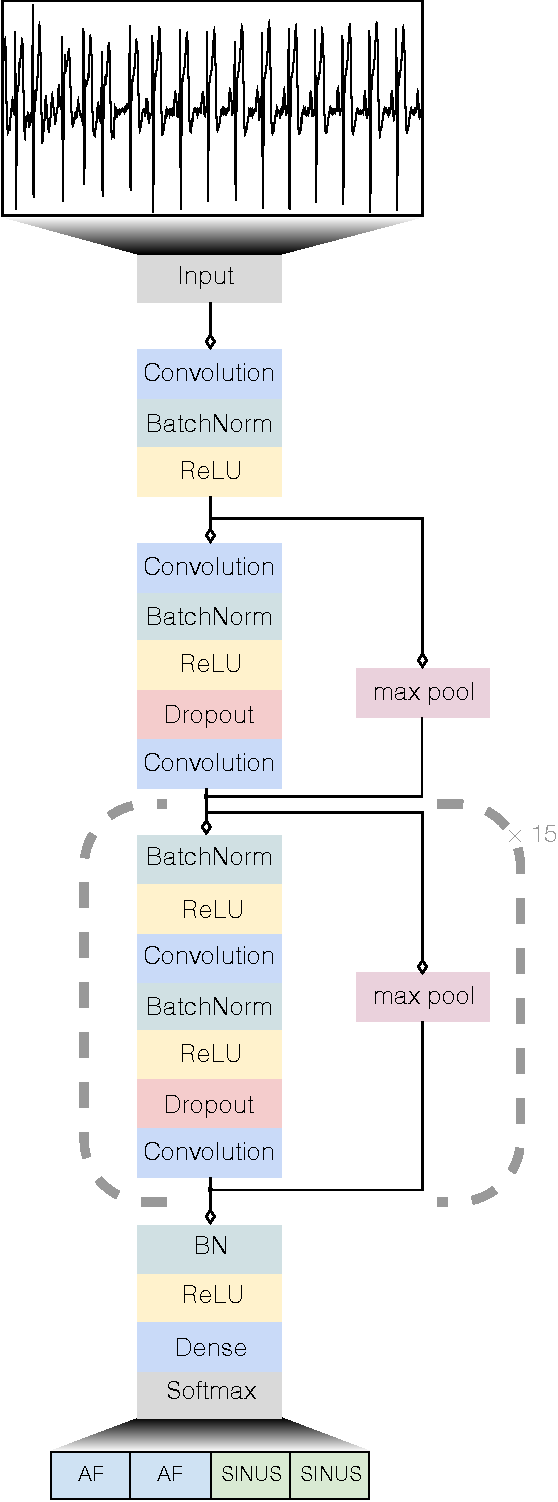
\includegraphics[width=0.4\textwidth]{arrhythmias/figures/ecg_network_full.pdf}
\caption{The architecture of the deep neural network consists of 33
         convolutional layers followed by a fully-connected layer and
         a softmax layer.}
\label{fig:arrhythmias:net}
\end{figure}

In order to make the optimization of such a network tractable, we employ
shortcut connections in a similar manner to those found in the Residual Network
architecture~\cite{he2016identity}. The shortcut connections between
neural-network layers optimize training by allowing information to propagate
well in very deep neural networks. Before the input is fed into the network, it
is normalized using a robust normalization strategy. The network consists of 16
residual blocks with 2 convolutional layers per block. The convolutional layers
all have a filter length of 16 and have 64$k$ filters, where $k$ starts out as
1 and is incremented every 4-th residual block. Every alternate residual block
subsamples its inputs by a factor of 2, thus the original input is ultimately
subsampled by a factor of $2^8$. When a residual block subsamples the input,
the corresponding shortcut connections also subsample their input using a Max
Pooling operation with the same subsample factor. 

Before each convolutional layer we apply Batch
Normalization~\cite{ioffe2015batch} and a rectified linear activation, adopting
the pre-activation block design~\cite{he2016deep}. The first and last layers of
the network are special-cased due to this pre-activation block structure. We
also apply Dropout~\cite{srivastava2014dropout} between the convolutional
layers and after the non-linearity. The final fully connected layer and softmax
activation produce a distribution over the 12 output classes for each
time-step.

We train the networks from scratch, initializing the weights of the
convolutional layers as in~\cite{he2015delving}. We use the
Adam~\cite{kingma2014adam} optimizer with the default parameters and reduce the
learning rate by a factor of 10 when the validation loss stops improving. We
save the best model as evaluated on the validation set during the optimization
process.

\section{Datasets}
\label{arrhythmia:sec:data}

\subsection*{Training}
We collect and annotate a dataset of 64,121 ECG records from 29,163 patients.
The ECG data is sampled at a frequency of 200 Hz and is collected from a
single-lead, noninvasive and  continuous monitoring device called the Zio Patch
which has a wear period up to 14 days \cite{turakhia2013diagnostic}. Each ECG
record in the training set is 30 seconds long and can contain more than one
rhythm type. Each record is annotated by a clinical ECG expert: the expert
highlights segments of the signal and marks it as corresponding to one of the
14 rhythm classes.

The 30 second records were annotated using a web-based ECG annotation tool
designed for this work. Label annotations were done by a group of Certified
Cardiographic Technicians who have completed extensive training in arrhythmia
detection and a cardiographic certification examination by Cardiovascular
Credentialing International. The technicians were guided through the interface
before they could annotate records. All rhythms present in a strip were labeled
from their corresponding onset to offset, resulting in full segmentation of the
input ECG data. To improve labeling consistency among different annotators,
specific rules were devised regarding each rhythm transition.

We split the dataset into a training and validation set. The training set
contains 90\% of the data. We split the dataset so that there is no patient
overlap between the training and validation sets (as well as the test set
described below).

\subsection*{Testing}

We collect a test set of 336 records from 328 unique patients. For the test
set, ground truth annotations for each record were obtained by a committee of
three board-certified cardiologists; there are three committees responsible for
different splits of the test set. The cardiologists discussed each individual
record as a group and came to a consensus labeling. For each record in the test
set we also collect 6 individual annotations from cardiologists not
participating in the group. This is used to assess performance of the model
compared to an individual cardiologist.

\subsection*{Rhythm Classes}
We identify 12 heart arrhythmias, sinus rhythm and noise for a total of 14
output classes. The arrhythmias are characterized by a variety of features.
Table~\ref{tab:rhythms} in the Appendix shows an example of each rhythm type we
classify. The noise label is assigned when the device is disconnected from the
skin or when the baseline noise in the ECG makes identification of the
underlying rhythm impossible.

The morphology of the ECG during a single heart-beat as well as the pattern of
the activity of the heart over time determine the underlying rhythm. In some
cases the distinction between the rhythms can be subtle yet critical for
treatment. For example two forms of second degree AV Block, Mobitz I
(Wenckebach) and Mobitz II (here referred to as AVB\_TYPE2) can be difficult to
distinguish. Wenckebach is considered benign and Mobitz II is considered
pathological, requiring immediate attention \cite{dubin1996rapid}. 

Table~\ref{tab:rhythms} in the Appendix also shows the number of unique
patients in the training (including validation) set and test set for each
rhythm type.

\section{Experimental Results}

\subsection*{Evaluation Metrics}
We use two metrics to measure model accuracy, using the cardiologist committee
annotations as the ground truth.

\textbf{Sequence Level Accuracy (F1):} We measure the average overlap between
the prediction and the ground truth sequence labels. For every record, a model
is required to make a prediction approximately once per second (every 256
samples). These predictions are compared against the ground truth annotation.

\textbf{Set Level Accuracy (F1):} Instead of treating the labels for a record
as a sequence, we consider the set of unique arrhythmias present in each 30
second record as the ground truth annotation. Set Level Accuracy, unlike
Sequence Level Accuracy, does not penalize for time-misalignment within a
record. We report the F1 score between the unique class labels from the ground
truth and those from the model prediction.

In both the Sequence and the Set case, we compute the metrics for each class
separately. We then compute aggregate results for AUC and F1 as the
class-frequency weighted mean.

\subsection*{Model and Cardiologist Performance}

We assess the cardiologist performance on the test set. Recall that each of the
records in the test set has a ground truth label from a committee of three
cardiologists as well as individual labels from a disjoint set of 6 other
cardiologists. To assess cardiologist performance for each class, we take the
average of all the individual cardiologist scores using the group label as the
ground truth annotation.

\begin{table}
\centering
\begin{small}
\begin{tabular}{r l l}
\toprule
                               & Sequence AUC & Set AUC \\
\midrule
Atrial Fibrillation \& Flutter & 0.975 & 0.959 \\
Atrio-ventricular Block        & 0.989 & 0.981 \\
Bigeminy                       & 0.998 & 0.997 \\
Ectopic Atrial Rhythm          & 0.908 & 0.935 \\
Idioventricular Rhythm         & 0.995 & 0.986 \\
Junctional Rhythm              & 0.985 & 0.980 \\
Noise                          & 0.985 & 0.958 \\
Sinus Rhythm                   & 0.976 & 0.981 \\
Supraventricular Tachycardia   & 0.972 & 0.940 \\
Trigeminy                      & 0.999 & 0.997 \\
Ventricular Tachycardia        & 0.995 & 0.981 \\
Wenckebach                     & 0.982 & 0.981 \\
\midrule
   Average                     & 0.979               & 0.974 \\
\bottomrule
\end{tabular}
\end{small}
\caption{The model AUC scores for each rhythm class and in aggregate.}
\label{tab:arrhythmias:model_auc}
\end{table}

Table~\ref{tab:arrhythmias:model_auc} gives the per class and aggregate AUC
scores. Our model achieves an AUC of greater than 0.90 for each of the 12
rhythm diagnoses, with an average AUC of 0.97. We also compute the sensitivity
at a specifity of 0.9 and vice versa in~\ref{tab:arrhythmias:sens_spec}.

\begin{table}
\centering
\begin{small}
\begin{tabular}{r l l}
\toprule
             & Sensitivity       & Specificity  \\
\midrule
Atrial Fibrillation \& Flutter & 0.923 & 0.914 \\
Atrio-ventricular Block        & 0.991 & 0.964 \\
Bigeminy                       & 1.000 & 0.997 \\
Ectopic Atrial Rhythm          & 0.754 & 0.665 \\
Idioventricular Rhythm         & 0.990 & 0.990 \\
Junctional Rhythm              & 0.982 & 0.959 \\
Noise                          & 0.965 & 0.968 \\
Sinus Rhythm                   & 0.934 & 0.946 \\
Supraventricular Tachycardia   & 0.958 & 0.925 \\
Trigeminy                      & 1.000 & 0.999 \\
Ventricular Tachycardia        & 1.000 & 0.981 \\
Wenckebach                     & 0.977 & 0.956 \\
\bottomrule
\end{tabular}
\end{small}
\caption{The maximum model sensitivity with specificity greater than 0.9 and
         vice versa.}
\label{tab:arrhythmias:sens_spec}
\end{table}

\begin{table}
\centering
\begin{small}
\begin{tabular}{r c c c c}
\toprule
    & \multicolumn{2}{c}{Sequence F1} & \multicolumn{2}{c}{Set F1} \\
\cmidrule{2-5}
 & Model & Cardiol. & Model & Cardiol. \\
\midrule
Atrial Fibrillation \& Flutter & 0.802 & 0.679 & 0.817 & 0.687 \\
Atrio-ventricular Block        & 0.850 & 0.769 & 0.830 & 0.756 \\
Bigeminy                       & 0.896 & 0.837 & 0.870 & 0.849 \\
Ectopic Atrial Rhythm          & 0.537 & 0.476 & 0.545 & 0.529 \\
Idioventricular Rhythm         & 0.751 & 0.632 & 0.818 & 0.720 \\
Junctional Rhythm              & 0.640 & 0.684 & 0.778 & 0.674 \\
Noise                          & 0.852 & 0.768 & 0.704 & 0.689 \\
Sinus Rhythm                   & 0.886 & 0.847 & 0.934 & 0.907 \\
Supraventricular Tachycardia   & 0.458 & 0.449 & 0.630 & 0.556 \\
Trigeminy                      & 0.909 & 0.843 & 0.870 & 0.816 \\
Ventricular Tachycardia        & 0.520 & 0.566 & 0.653 & 0.769 \\
Wenckebach                     & 0.714 & 0.593 & 0.806 & 0.736 \\
\midrule
Average	                       & 0.808 & 0.750 & 0.809 & 0.778 \\
\bottomrule
\end{tabular}
\end{small}
\caption{The F1 score for the sequence and set-level metrics comparing the
         model and the average of six individual cardiologist to the committee
         consensus ground truth.}
\label{tab:arrhythmias:model_cardiologist_f1}
\end{table}

Table~\ref{tab:arrhythmias:model_cardiologist_f1} shows the breakdown of both
cardiologist and model sequence and set F1 across the different rhythm classes.
The model outperforms the average cardiologist performance on most rhythms,
noticeably outperforming the cardiologists in the AV Block set of arrhythmias
which includes Mobitz I (Wenckebach), Mobitz II and complete heart block (both
categorized as Atrio-ventricular Block). This is especially useful given the
severity of second and third degree heart block and the importance of
distinguishing these two from Wenckebach which is usually considered benign.
The model also outperforms the cardiologist average accross all rhythm classes
for both the sequence and set F1 score.

\begin{figure}
\centering
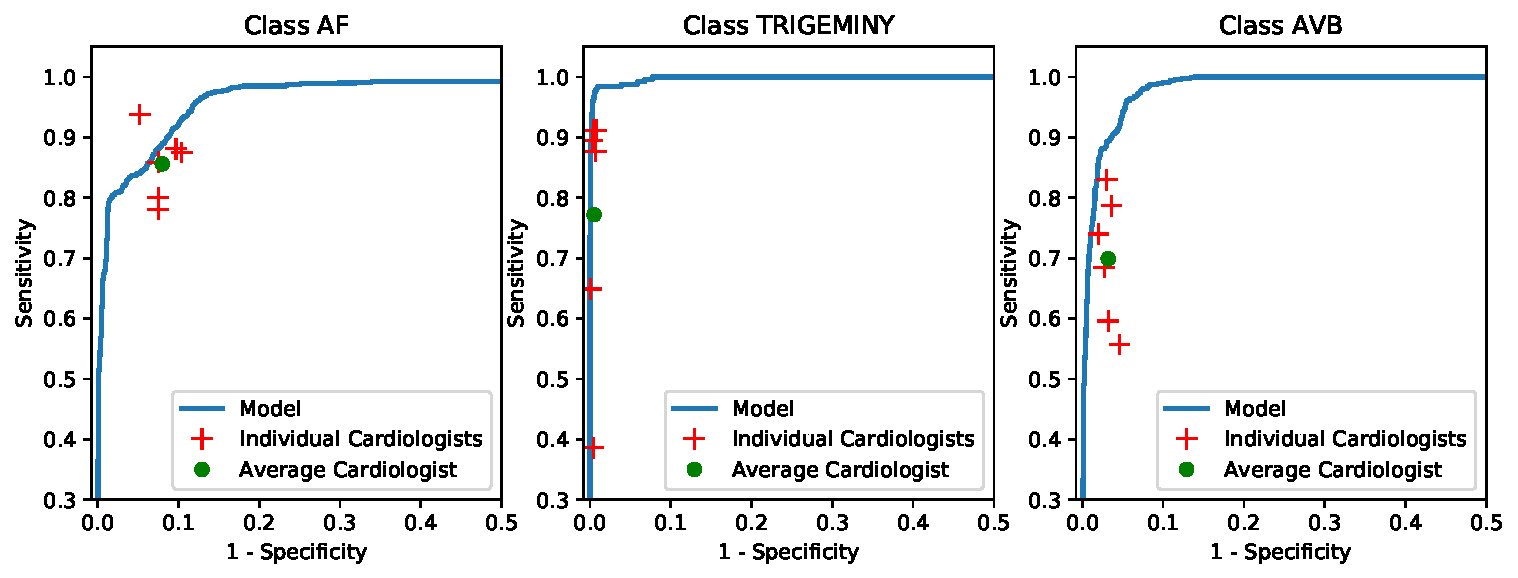
\includegraphics[width=1.0\textwidth]{arrhythmias/figures/roc_curve.pdf}
\caption{Receiver operating characteristic curves at the sequence level for
    atrial fibrillation and flutter (AF), trigeminy and atrioventricular block
    (AVB).}
\label{fig:arrhythmias:roc_curve}
\end{figure}

Figures~\ref{fig:arrhythmias:roc_curve} and
\ref{fig:arrhythmias:prec_recall_curve} show the models performance at various
operating thresholds on an ROC and precision-recall curve respectively. We show
here three arrhythmias taken from one-third of the test set. We also compute
and plot the operating point for the six individual cardiologists who annotated
that third of the test set. The model outperforms almost all of the individual
cardiologists. We see the same behaviour for the other rhythm classes not shown
here.

\begin{figure}
\centering
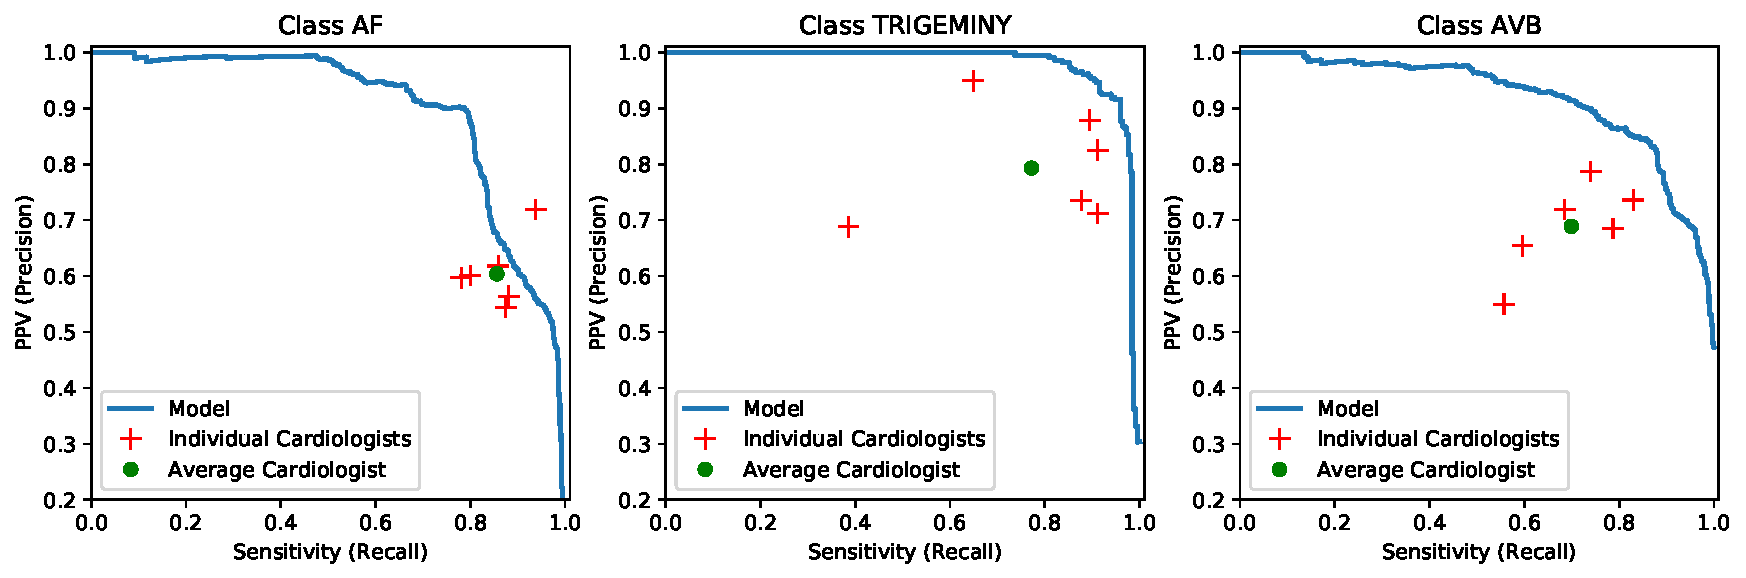
\includegraphics[width=1.0\textwidth]{arrhythmias/figures/prec_recall_curve.pdf}
    \caption{Precision-recall curves at the sequence level for atrial
    fibrillation and flutter (AF), trigeminy and atrioventricular block (AVB).}
\label{fig:arrhythmias:prec_recall_curve}
\end{figure}

\section{Analsysis}

The model outperforms the average cardiologist score on both the sequence and
the set F1 metrics. Figure~\ref{fig:confusion} shows a confusion matrix of the
model predictions on the test set. Many arrhythmias are confused with the sinus
rhythm. We expect that part of this is due to the sometimes ambiguous location
of the exact onset and offset of the arrhythmia in the ECG record.

\begin{figure}
\begin{subfigure}{.5\textwidth}
  \centering
  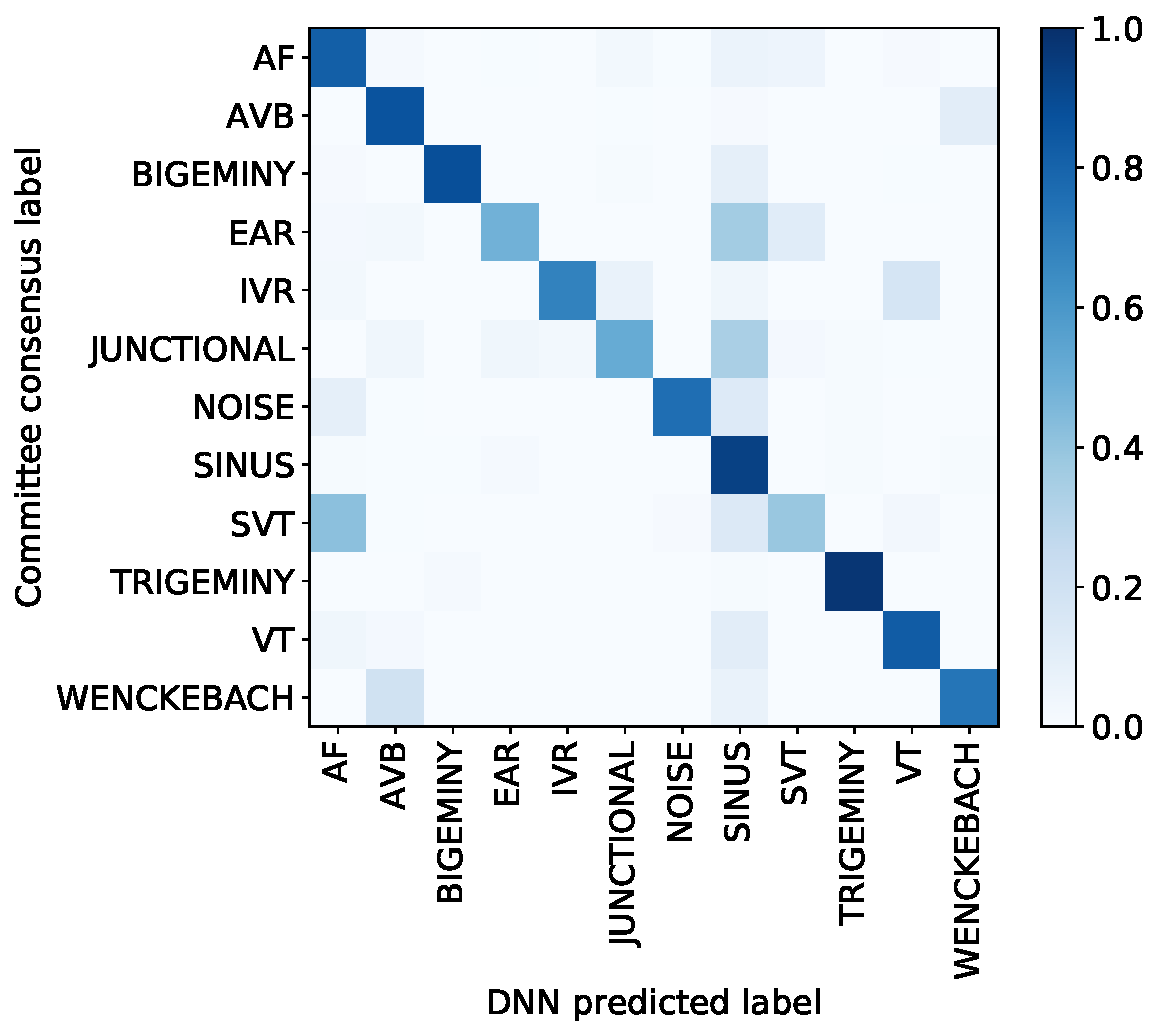
\includegraphics[width=0.9\linewidth]{arrhythmias/figures/model_confusions.pdf}
  \caption{Model}
  \label{fig:arrhythmia:model_confusion}
\end{subfigure}
\begin{subfigure}{.5\textwidth}
  \centering
  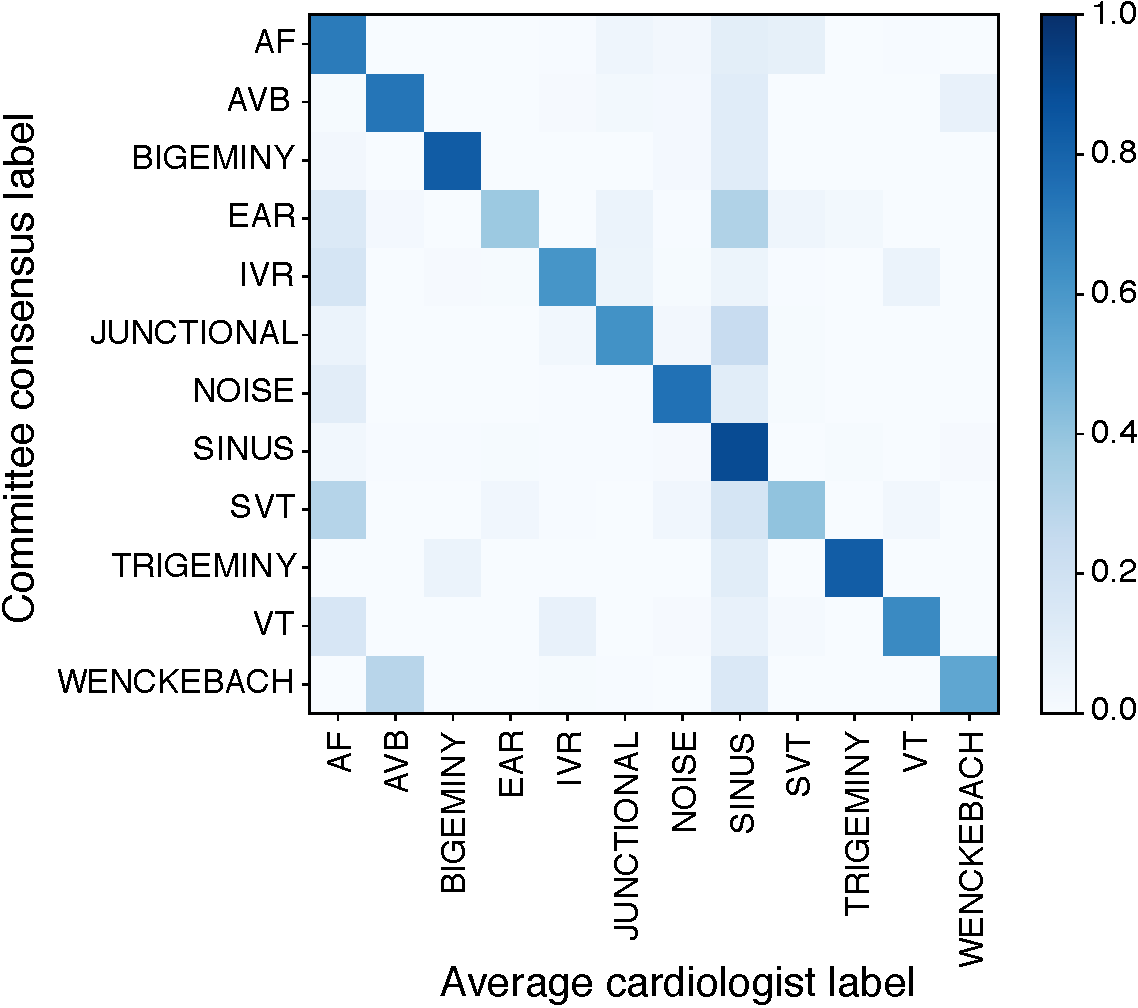
\includegraphics[width=0.9\linewidth]{arrhythmias/figures/human_confusions.pdf}
  \caption{Individual Cardiologists}
  \label{fig:arrhythmia:human_confusion}
\end{subfigure}
\caption{Confusion matrices for the model and individual cardiologist
         predictions with the committee consensus annotations as ground
         truth.}
\end{figure}

Often the mistakes made by the model are understandable. For example, confusing
Wenckebach and AVB\_Type2 makes sense given that the two rhythms in general
have very similar ECG morphologies. Similarly, Supraventricular Tachycardia
(SVT) and Atrial Fibrillation (AFIB) are often confused with Atrial Flutter
(AFL) which is understandable given that they are all atrial arrhythmias. We
also note that Idioventricular Rhythm (IVR) is sometimes mistaken as
Ventricular Tachycardia (VT), which again makes sense given that the two only
differ in heart-rate and are difficult to distinguish close to the 100 beats
per minute delineation.

One of the most common confusions is between Ectopic Atrial Rhythm (EAR) and
the sinus rhythm. The main distinguishing criteria for this rhythm is an
irregular P wave. This can be subtle to detect especially when the P wave has a
small amplitude or when noise is present in the signal.

\section{Conclusion}

We develop a model which exceeds the cardiologist performance in detecting a
wide range of heart arrhythmias from single-lead ECG records. Key to the
performance of the model is a large annotated dataset and a very deep
convolutional network which can map a sequence of ECG samples to a sequence of
arrhythmia annotations. 

On the clinical side, future work should investigate extending the set of
arrhythmias and other forms of heart disease which can be automatically
detected with high-accuracy from single or multiple lead ECG records. For
example we do not detect Ventricular Flutter or Fibrillation. We also do not
detect Left or Right Ventricular Hypertrophy, Myocardial Infarction or a number
of other heart diseases which do not necessarily exhibit as arrhythmias. Some
of these may be difficult or even impossible to detect on a single-lead ECG but
can often be seen on a multiple-lead ECG.

Given that more than 300 million ECGs are recorded annually, high-accuracy
diagnosis from ECG can save expert clinicians and cardiologists considerable
time and decrease the number of misdiagnoses. Furthermore, we hope that this
technology coupled with low-cost ECG devices enables more widespread use of the
ECG as a diagnostic tool in places where access to a cardiologist is difficult.


\chapter{First-pass Speech Recognition}

\section{Introduction}
\label{sec:first_pass:introduction}

Modern large vocabulary continuous speech recognition (LVCSR) systems are
complex and difficult to modify. Much of this complexity stems from the
paradigm of modeling words as sequences of sub-phonetic states with hidden
Markov models (HMMs). HMM-based systems require carefully-designed training
recipes to construct consecutively more complex HMM recognizers. The overall
difficulty of building, understanding, and modifying HMM-based LVCSR systems
has limited progress in speech recognition and isolated it from many advances
in related fields. 

Previous work demonstrated an HMM-free approach for training a speech
recognizer \cite{graves2014}. The authors use a neural network to directly
predict transcript characters given the audio of an utterance. This approach
discards many of the assumptions present in modern HMM-based LVCSR systems in
favor of treating speech recognition as a direct sequence transduction problem.
The approach trains a neural network using the connectionist temporal
classification (CTC) loss function, which amounts to maximizing the likelihood
of an output sequence by efficiently summing over all possible input-output
sequence alignments.  Using CTC the authors were able to train a neural network
to predict the character sequence of test utterances with a character error
rate (CER) under 10\% on the Wall Street Journal LVCSR corpus. While impressive
in its own right, these results are not yet competitive with existing HMM-based
systems in terms of word error rate (WER). Good word-level performance in
speech recognition often depends heavily upon a language model to provide a
prior probability over likely word sequences. 

To integrate language model information during decoding, the probabilities from
the CTC-trained neural network are used to rescore a lattice or n-best
hypothesis list generated by a state-of-the-art HMM-based system
\cite{graves2014}. This introduces a potentially confounding factor because an
n-best list constrains the set of possible transcriptions significantly.
Additionally, it results in an overall system which still relies on HMM speech
recognition infrastructure to achieve the final results. In contrast, we
present \emph{first-pass} decoding results which use a neural network and
language model to decode from scratch, rather than re-ranking an existing set
of hypotheses.

We describe a decoding algorithm which directly integrates a language model
with CTC-trained neural networks to search through the space of possible word
sequences. Our first-pass decoding algorithm enables CTC-trained models to
benefit from a language model without relying on an existing HMM-based system
to generate a word lattice. This removes the lingering dependence on
HMM-centric speech recognition toolkits and enables us to achieve fairly
competitive WER results with only a neural network and $n$-gram language model.

Deep neural networks (DNNs) are the most widely used neural network
architecture for speech recognition \cite{hinton2012}. DNNs are a fairly
generic architecture for classification and regression problems. In HMM-based
LVCSR systems, DNNs act as acoustic models by predicting the HMM's hidden state
given the acoustic input for a point in time. However, in such HMM-DNN systems
the temporal reasoning about an output sequence takes place within the HMM
rather than the neural network. CTC training of neural networks forces the
network to model output sequence dependencies rather than reasoning about
single time frames independently from others. To better handle such temporal
dependencies previous work with CTC used long short term memory (LSTM)
networks. LSTM is a neural network architecture was originally designed to
prevent the vanishing gradient problem of sigmoidal DNNs or temporally
recurrent deep neural networks (RDNNs) \cite{hochreiter1997}.

Our work uses RDNNs instead of LSTMs as a neural network architecture. RDNNs
are simpler overall, because there are only dense weight matrix connections
between subsequent layers. This simpler architecture is more amenable to
graphics processing unit (GPU) computing which can significantly reduce
training times. Recent work shows that with rectifier nonlinearities DNNs can
perform well in DNN-HMM systems without suffering from vanishing gradient
problems during optimization \cite{dahl2013, zeiler2013, maas2013}. This makes
us hopeful that RDNNs with rectifier nonlinearities may be able to perform
comparably to LSTMs which are specially engineered to avoid vanishing
gradients.

\section{Model}
\label{sec:first_pass:model}

We train neural networks using the CTC loss function to do maximum
likelihood training of letter sequences given acoustic features as
input. We consider a single utterance as a training example consisting
of an acoustic feature matrix $X$ and word transcription $Y$. The CTC
objective function maximizes the log probability $\log p(Y \mid X)$. We
reserve a full exposition of the loss function here because our
formulation follows exactly the previous work on using CTC to predict
the characters of an utterance transcription~\cite{graves2014, graves2006}. 

\subsection{Deep Neural Networks}
\label{sec:first_pass:model:dnn}

With the loss function fixed we must next define how we compute $p(c \mid
x_t)$, the predicted distribution over output characters $c$ given the audio
features $x_t$ at time $t$. While many function approximators are possible for
this task, we choose as our most basic model a DNN. A DNN computes the
distribution $p(c \mid x_t)$ using a series of hidden layers followed by an output
layer. Given an input vector $x_t$ the first hidden layer activations are a
vector computed as,
\begin{align*}
  h^{(1)} = \sigma(W^{(1)T} x_t + b^{(1)}).
\end{align*}
The matrix $W^{(1)}$ and vector $b^{(1)}$ are the weight matrix and bias vector
for the layer. The function $\sigma(\cdot)$ is a point-wise nonlinearity. We
use rectifier nonlinearities and thus choose, $\sigma(z) = \max (z, 0)$.

DNNs can have arbitrarily many hidden layers. After the first hidden
layer, the hidden activations $h^{(i)}$ for layer $i$ are computed as,
\begin{align*}
  h^{(i)} = \sigma(W^{(i)T} h^{(i-1)} + b^{(i)}).
\end{align*}

To obtain a proper distribution over the set of possible characters $c$ the
final layer of the network is a \emph{softmax} output layer of the form,
\begin{align*}
  p(c=c_k \mid x_t) = \frac{\exp(- ( W^{(s)T}_k h^{(i-1)} + b^{(s)}_k))}
  {\sum_j \exp(- ( W^{(s)T}_j h^{(i-1)} + b^{(s)}_j))},
\end{align*}
where $W^{(s)}_k$ is the $k$'th column of the output weight matrix $W^{(s)}$
and $b^{(s)}_k$ is a scalar bias term. 

We can compute a subgradient for all parameters of the DNN given a training
example and thus utilize gradient-based optimization techniques. Note that this
same DNN formulation is commonly used in DNN-HMM models to predict a
distribution over senones instead of characters.

\subsection{Recurrent Deep Neural Networks}

A transcription $W$ has many temporal dependencies which a DNN may not
sufficiently capture. At each timestep $t$ the DNN computes its output using
only the input features $x_t$, ignoring previous hidden representations and
output distributions. To enable better modeling of the temporal dependencies
present in a problem, we use a RDNN. In a RDNN we select one hidden layer $j$
to have a temporally recurrent weight matrix $W^{(f)}$ and compute the layer's
hidden activations as,
\begin{align*}
  h^{(j)}_t = \sigma(W^{(j)T} h^{(j-1)}_t +  W^{(f)T} h^{(j)}_{t-1} + b^{(j)}).
\end{align*}
Note that we now make the distinction $h^{(j)}_t$ for the hidden activation
vector of layer $j$ at timestep $t$ since it now depends upon the activation
vector of layer $j$ at time $t-1$.

When working with RDNNs, we found it important to use a modified version of the
rectifier nonlinearity. This modified function selects $\sigma(z) = \min( \max
(z, 0), 20)$ which clips large activations to prevent divergence during network
training. Setting the maximum allowed activation to 20 results in the clipped
rectifier acting as a normal rectifier function in all but the most extreme
cases.

Aside from these changes, computations for a RDNN are the same as those in a
DNN as described in \ref{sec:first_pass:model:dnn}. Like the DNN, we can
compute a subgradient for a RDNN using a method sometimes called
backpropagation through time. In our experiments we always compute the gradient
completely through time rather than truncating to obtain an approximate
subgradient.

\subsection{Bi-Directional Recurrent Deep Neural Networks}

While forward recurrent connections reflect the temporal nature of the audio
input, a perhaps more powerful sequence transduction model is a BRDNN, which
maintains state both forwards and backwards in time. Such a model can integrate
information from the entire temporal extent of the input features when making
each prediction. We extend the RDNN to form a BRDNN by again choosing a
temporally recurrent layer $j$. The BRDNN creates both a forward and backward
intermediate hidden representation which we call $h_t^{(f)}$ and $h_t^{(b)}$
respectively. 

We use the temporal weight matrices $W^{(f)}$ and $W^{(b)}$ to propagate
$h_t^{(f)}$ forward in time and $h_t^{(b)}$ backward in time respectively. We
update the forward and backward components via the equations,
\begin{align*}
    h^{(f)}_t &= \sigma(W^{(j)T} h^{(j-1)}_t +  W^{(f)T} h^{(f)}_{t-1} + b^{(j)}), \\
    h^{(b)}_t &= \sigma(W^{(j)T} h^{(j-1)}_t +  W^{(b)T} h^{(b)}_{t+1} + b^{(j)}).
\end{align*}

Note that the recurrent forward and backward hidden representations are
computed entirely independently from each other. As with the RDNN we use the
modified nonlinearity function $\sigma(z) = \min( \max (z,0), 20)$. To obtain
the final representation $h^{(j)}_t$ for the layer we sum the two temporally
recurrent components,
\begin{align}
\begin{split}
  h^{(j)}_t = h^{(f)}_t + h^{(b)}_t.
\end{split}
\end{align}

Aside from this change to the recurrent layer the BRDNN computes its output
using the same equations as the RDNN. As for other models, we can compute a
subgradient for the BRDNN directly to perform gradient-based optimization.

\section{Decoding}
\label{sec:first_pass:decoding}

%%% NOTATION KEY:
% \Sigma is extended alphabet including blank
% S and s_t is sequence and sequence item at time t including blank char
% T is time, 
% x_t is input at time t, X is full audio input of length T
% W is full word output
% \ell is character label prefix not including blanks
% p(c; x_t) is output of BDRNN at time t

Assuming an input of length $T$, the output of the neural network will be $p(c;
x_t)$ for $t = 1,\ldots,T$. Again, $p(c; x_t)$ is a distribution over possible
characters in the alphabet $\Sigma$, which includes the blank symbol, given
audio input $x_t$. In order to recover a character string from the output of
the neural network, as a first approximation, we take the \texttt{argmax} at
each time step. Let $S = (s_1,\ldots,s_T)$ be the character sequence where $s_t
= \argmax_{c \in \Sigma} p(c; x_t)$. The sequence $S$ is mapped to a
transcription by collapsing repeat characters and removing blanks. This gives a
sequence which can be scored against the reference transcription using both CER
and WER.

This first approximation lacks the ability to include the constraint of either
a lexicon or a language model. We propose a generic algorithm which is capable
of incorporating such constraints. Taking $X$ to be the acoustic input of time
$T$, we seek a transcription $W$ which maximizes the probability,
\begin{equation}
  \label{eq:joint} p_{\text{net}}(W ; X) p_{\text{lm}}(W).  
\end{equation} 
Here the overall probability of the transcription is modeled as the product of
two factors: $p_{\text{net}}$ given by the network and $p_{\text{lm}}$ given by
a language model prior. In practice the prior $p_{\text{lm}}(W)$, when given by
an $n$-gram language model, is too constraining and thus we down-weight it and
include a word insertion penalty (or bonus) as
\begin{equation}\label{eq:amlm}
    p_{\text{net}}(W ; X) p_{\text{lm}}(W)^\alpha |W|^\beta.
\end{equation}
Alogrithm \ref{alg:decode} attempts to find a word string $W$ which maximizes
equation \ref{eq:amlm}.
\begin{algorithm}[bt]
  \caption{Prefix Beam Search: The algorithm initializes the previous set of
prefixes $A_\text{prev}$ to the empty string. For each time step and every
prefix $\ell$ currently in $A_\text{prev}$, we propose adding a character from the
alphabet $\Sigma$ to the prefix. If the character is a blank, we do not extend
the prefix. If the character is a space, we incorporate the language model
constraint. Otherwise we extend the prefix and incorporate the output of the
network. All new active prefixes are added to $A_\text{next}$. We then set
$A_\text{prev}$ to include only the $k$ most probable prefixes of $A_\text{next}$.
The output is the $1$ most probable transcript, although the this can easily
be extended to return an $n$-best list.}\label{alg:decode}
  \begin{algorithmic}
    \State $p_b(\emptyset; x_{1:0}) \gets 1,\; p_{nb}(\emptyset; x_{1:0}) \gets 0$
    \State $A_{\text{prev}} \gets \{\emptyset\}$ 
    \For {$t = 1, \ldots, T$}
      \State $A_{\text{next}} \gets \{\}$
      \For {$\ell \; \text{\bf in} \; A_{\text{prev}}$}
	\For {$c \; \text{\bf in} \; \Sigma$}
	  \If {$c = \text{blank}$}
	    \State $p_b(\ell; x_{1:t}) \gets p(\text{blank}; x_t) 
		(p_b(\ell ; x_{1:t-1}) + p_{nb}(\ell ; x_{1:t-1}))$
	    \State $\mbox{add } \ell \mbox{ to } A_{\text{next}}$
	  \Else
	    \State $\ell^+ \gets \mbox{concatenate }\ell \mbox{ and } c$
	    \If {$c = \ell_\text{end}$}
	      \State $p_{nb}(\ell^+; x_{1:t}) \gets p(c; x_t)p_b(\ell ; x_{1:t-1})$
	      \State $p_{nb}(\ell; x_{1:t}) \gets p(c; x_t)p_b(\ell ; x_{1:t-1})$
	    \ElsIf {$c = \text{space}$}
	    \State $p_{nb}(\ell^+; x_{1:t}) \gets p(W(\ell^+)| W(\ell))^\alpha 
		p(c; x_t)(p_b(\ell ; x_{1:t-1}) + p_{nb}(\ell ; x_{1:t-1}))$
	    \Else
	      \State $p_{nb}(\ell^+; x_{1:t}) \gets p(c; x_t)
		(p_b(\ell; x_{1:t-1}) + p_{nb}(\ell; x_{1:t-1}))$
	    \EndIf
	    \If {$\ell^+ \; \text{\bf not in} \; A_\text{prev}$}
	      \State $p_{b}(\ell^+; x_{1:t}) \gets p(\text{blank}; x_t)
		(p_b(\ell^+; x_{1:t-1}) + p_{nb}(\ell^+; x_{1:t-1}))$
	      \State $p_{nb}(\ell^+; x_{1:t}) \gets p(c; x_t)p_{nb}(\ell^+; x_{1:t-1})$
	    \EndIf
	    \State $\mbox{add } \ell^+ \mbox{ to } A_{\text{next}}$
	  \EndIf
	\EndFor
      \EndFor
      \State $A_{\text{prev}} \gets k 
	\text{ most probable prefixes in } A_{\text{next}}$
    \EndFor
    \State \Return $1 \text{ most probable prefix in } A_{\text{prev}}$
  \end{algorithmic}
\end{algorithm}
The algorithm maintains two separate probabilities for each prefix,
$p_{b}(\ell; x_{1:t})$ and $p_{nb}(\ell; x_{1:t})$. Respectively, these are the
probability of the prefix $\ell$ ending in blank or not ending in blank given
the first $t$ time steps of the audio input $X$.

The sets $A_{\text{prev}}$ and $A_{\text{next}}$ maintain a list of active
prefixes at the previous time step and proposed prefixes at the next time step
respectively. Note that the size of $A_{\text{prev}}$ is never larger than the
beam width $k$. The overall probability of a prefix is the product of a word
insertion term and the sum of the blank and non-blank ending probabilities,
\begin{equation}\label{eq:prefixprob}
  p(\ell; x_{1:t}) = (p_b(\ell; x_{1:t}) + p_{nb}(\ell; x_{1:t})) |W(\ell)|^\beta,
\end{equation}
where $W(\ell)$ is the set of words in the sequence $\ell$. When taking the $k$
most probable prefixes of $A_{\text{next}}$, we sort each prefix using the
probability given by equation \ref{eq:prefixprob}.

The variable $\ell_{\text{end}}$ is the last character in the label sequence
$\ell$. The function $W(\cdot)$, which converts $\ell$ into a string of words,
segments the sequence $\ell$ at each space character and truncates any
characters trailing the last space. 

We incorporate a lexicon or language model constraint by including the
probability $p(W(\ell^+) | W(\ell))$ whenever the algorithm proposes appending
a space character to $\ell$. By setting $p(W(\ell^+) | W(\ell))$ to $1$ if the
last word of $W(\ell^+)$ is in the lexicon and $0$ otherwise, the probability
acts as a constraint forcing all character strings $\ell$ to consist of only
words in the lexicon.  Furthermore, $p(W(\ell^+) | W(\ell))$ can represent a
$n$-gram language model by considering only the last $n-1$ words in $W(\ell)$.  


\section{Experiments}

We evaluate our approach on the 81 hour Wall Street Journal (WSJ) news article
dictation corpus (available in the LDC catalog as LDC94S13B and LDC93S6B). Our
training set consists of 81 hours of speech from 37,318 utterances. The basic
preparation of transforming the LDC-released corpora into training and test
subsets follows the Kaldi speech recognition toolkit's s5
recipe~\cite{povey2011}. However, we did not apply much of the text
normalization used to prepare transcripts for training an HMM system. Instead
we simply drop unnecessary transcript notes like lexical stress, keeping
transcribed word fragments and acronym punctuation marks. We can safely discard
much of this normalization because our approach does not rely on a lexicon or
pronunciation dictionary, which cause problems especially for word fragments.
Our language models are the standard models released with the WSJ corpus
without lexical expansion. We used the `dev93' evaluation subset as a
development set and report final test set performance on the `eval92'
evaluation subset. Both subsets use the same 20k word vocabulary. The language
model used for decoding is constrained to this same 20k word vocabulary.

The input audio was converted into log-Mel filterbank features with 23
frequency bins. A context window of +/- 10 frames were concatenated to form a
final input vector of size 483. We did not perform additional feature
preprocessing or feature-space speaker adaptation.  Our output alphabet
consists of 32 classes, namely the blank symbol ``\_'', 26 letters, 3
punctuation marks (apostrophe, ., and -) as well as tokens for noise and space. 

\subsection{First-Pass Decoding with a Language Model}

We trained a BRDNN with 5 hidden layers, all with 1824 hidden units, for a
total of 20.9M free parameters. The third hidden layer of the network has
recurrent connections. Weights in the network are initialized from a uniform
random distribution scaled by the weight matrix's input and output layer
size~\cite{glorot2011}. We use the Nesterov accelerated gradient optimization
algorithm~\cite{sutskever2013} with initial learning rate $10^{-5}$, and
maximum momentum 0.95. After each full pass through the training set we divide
the learning rate by 1.2 to ensure the overall learning rate decreases over
time. We train the network for a total of 20 passes over the training set,
which takes about 96 hours using our Python GPU implementation.  For decoding
with prefix search we use a beam size of 200 and cross-validate with a held-out
set to find a good setting of the parameters $\alpha$ and $\beta$.
Table~\ref{tab:first_pass:res_decode} shows word and character error rates for
multiple approaches to decoding with this trained BRDNN.

\begin{table}
\centering
\begin{tabular}{lrr}
\toprule
Model & CER & WER\\
\midrule
No LM         & 10.0 & 35.8 \\
Dictionary LM & 8.5  & 24.4 \\
Bigram LM     & 5.7  & 14.1 \\
\bottomrule
\end{tabular}
\caption{Word error rate (WER) and character error rate (CER) results
  for a BDRNN trained with the CTC loss function.}
\label{tab:first_pass:res_decode}
\end{table}

Without any sort of language constraint WER is quite high, despite the fairly
low CER. This is consistent with our observation that many mistakes at the
character level occur when a word appears mostly correct but does not conform
to the highly irregular orthography of English. Prefix-search decoding using
the 20k word vocabulary as a prior over possible character sequences results in
a substantial WER improvement, but changes the CER relatively little. Comparing
the CERs of the no LM and dictionary LM approaches again demonstrates that
without an LM the characters are mostly correct but are distributed across many
words which increases WER. A large relative drop in both CER and WER occur when
we decode with a bigram LM. Performance of the bigram LM model demonstrates
that CTC-trained systems can attain competitive error rates without relying on
a lattice or n-best list generated by an existing speech system.

\subsection{The Effect of Recurrent Connections}

Previous experiments with DNN-HMM systems found minimal benefits from recurrent
connections in DNN acoustic models. It is natural to wonder whether recurrence,
and especially bi-directional recurrence, is an essential aspect of our
architecture. To evaluate the impact of recurrent connections we compare the
train and test CERs of DNN, RDNN, and BRDNN models while roughly controlling
for the total number of free parameters in the model.
Table~\ref{tab:first_pass:res_recurrence} shows the results for each type of
architecture. 

\begin{table}
\centering
\begin{tabular}{lrrr}
\toprule
Model & Parameters (M) & Train CER & Test CER \\
\midrule
DNN   & 16.8 & 3.8 & 22.3 \\
RDNN  & 22.0 & 4.2 & 13.5 \\
BRDNN & 20.9 & 2.8 & 10.7 \\
\bottomrule
\end{tabular}
\caption{Train and test set CER results for a DNN without recurrence, an RDNN,
         and a BRDNN.}
\label{tab:first_pass:res_recurrence}
\end{table}

Both variants of recurrent models show substantial test set CER improvements
over the non-recurrent DNN model. Note that we report performance for a DNN of
only 16.8M total parameters which is smaller than the total number of
parameters used in both the RDNN and BRDNN models. We found that larger DNNs
performed worse on the test set, suggesting that DNNs may be more prone to
over-fitting for this task. Although the BRDNN has fewer parameters than the
RDNN it performs better on both the training and test sets. Again this suggests
that the architecture itself drives improved performance rather than the total
number of free parameters. Conversely, because the gap between bi-directional
recurrence and single recurrence is small relative to a non-recurrent DNN,
on-line speech recognition using a singly recurrent network may be feasible
without overly damaging performance.

\section{Conclusion}

We presented a decoding algorithm which enables first-pass LVCSR with a
language model for CTC-trained neural networks. This decoding approach removes
the lingering dependence on HMM-based systems found in previous work.
Furthermore, first-pass decoding demonstrates the capabilities of a CTC-trained
system without the confounding factor of potential effects from pruning the
search space via a provided lattice. While our results do not outperform the
best HMM-based systems on the WSJ corpus, they demonstrate the promise of
CTC-based speech recognition systems.

Our experiments with the BRNN further simplify the infrastructure needed to
create CTC-based speech recognition systems. The BRNN is overall a less complex
architecture than LSTMs and can relatively easily be made to run on GPUs since
large matrix multiplications dominate the computation. However, our experiments
suggest that recurrent connections are critical for good performance.
Bi-directional recurrence helps beyond unidirectional recurrence but could be
sacrificed in cases that require low-latency, online speech recognition. Taken
together with previous work on CTC-based LVCSR, we believe there is an exciting
path forward for high quality LVCSR without the complexity of HMM-based
infrastructure.


\chapter{Deep Speech: Scaling Up End-to-end Speech Recognition}

\section{Introduction}
\label{sec:deepspeech:introduction}

Top speech recognition systems rely on sophisticated pipelines composed of
multiple algorithms and hand-engineered processing stages. In this paper, we
describe an end-to-end speech system, called ``Deep Speech'', where deep
learning supersedes these processing stages. Combined with a language model,
this approach achieves higher performance than traditional methods on hard
speech recognition tasks while also being much simpler. These results are made
possible by training a large recurrent neural network (RNN) using multiple GPUs
and thousands of hours of data. Because this system learns directly from data,
we do not require specialized components for speaker adaptation or noise
filtering. In fact, in settings where robustness to speaker variation and noise
are critical, our system excels: Deep Speech outperforms previously published
methods on the Switchboard Hub5'00 corpus, achieving 16.0 WER, and performs
better than commercial systems in noisy speech recognition tests.

Traditional speech systems use many heavily engineered processing stages,
including specialized input features, acoustic models, and Hidden Markov Models
(HMMs). To improve these pipelines, domain experts must invest a great deal of
effort tuning their features and models. The introduction of deep learning
algorithms~\cite{lee2009, mohamed2011, hinton2012, dahl2011a} has improved
speech system performance, usually by improving acoustic models.  While this
improvement has been significant, deep learning still plays only a limited role
in traditional speech pipelines. As a result, to improve performance on a task
such as recognizing speech in a noisy environment, one must laboriously
engineer the rest of the system for robustness. In contrast, our system applies
deep learning end-to-end using recurrent neural networks.  We take advantage of
the capacity provided by deep learning systems to learn from large datasets to
improve our overall performance. Our model is trained end-to-end to produce
transcriptions and thus, with sufficient data and computing power, can learn
robustness to noise or speaker variation on its own.

Tapping the benefits of end-to-end deep learning, however, poses several
challenges: (i) we must find innovative ways to build large, labeled training
sets and (ii) we must be able to train networks that are large enough to
effectively utilize all of this data. One challenge for handling labeled data
in speech systems is finding the alignment of text transcripts with input
speech. This problem has been addressed by Graves, Fern\'{a}ndez, Gomez and
Schmidhuber~\cite{graves2006}, thus enabling neural networks to easily consume
unaligned, transcribed audio during training. Meanwhile, rapid training of
large neural networks has been tackled by Coates et
al.~\cite{coates2013cotshpc}, demonstrating the speed advantages of multi-GPU
computation. We aim to leverage these insights to fulfill the vision of a
generic learning system, based on large speech datasets and scalable RNN
training, that can surpass more complicated traditional methods. This vision
is inspired partly by the work of Lee~et.~al.~\cite{lee2009} who
applied early unsupervised feature learning techniques to replace hand-built
speech features.

We have chosen our RNN model specifically to map well to GPUs and we use a
novel model partition scheme to improve parallelization. Additionally, we
propose a process for assembling large quantities of labeled speech data
exhibiting the distortions that our system should learn to handle. Using a
combination of collected and synthesized data, our system learns robustness to
realistic noise and speaker variation (including Lombard
Effect~\cite{junqua1993lombard}). Taken together, these ideas suffice to build
an end-to-end speech system that is at once simpler than traditional pipelines
yet also performs better on difficult speech tasks. Deep Speech achieves a word
error rate of 16.0 on the full Switchboard Hub5'00 test set---the best
published result. Further, on a new noisy speech recognition dataset of our own
construction, our system achieves a word error rate of 19.1 where the best
commercial systems achieve 30.5 error.

\section{Related Work}
\label{sec:deepspeech:related}

Several parts of our work are inspired by previous results. Neural network
acoustic models and other connectionist approaches were first introduced to
speech pipelines in the early 1990s~\cite{bourlard93, renals1994, ellis1999}.
These systems, similar to DNN acoustic models~\cite{mohamed2011, hinton2012,
dahl2011a}, replace only one stage of the speech recognition pipeline.
Mechanically, our system is similar to other efforts to build end-to-end speech
systems from deep learning algorithms. For example,
Graves~et~al.~\cite{graves2006} have previously introduced the ``Connectionist
Temporal Classification'' (CTC) loss function for scoring transcriptions
produced by RNNs and, with LSTM networks, have previously applied this approach
to speech~\cite{graves2014}. We similarly adopt the CTC loss for part of our
training procedure but use much simpler recurrent networks with
rectified-linear activations~\cite{glorot2011, maas2013, nair2010}. Our
recurrent network is similar to the bidirectional RNN used by Hannun et
al.~\cite{hannun2014firstpass}, but with multiple changes to enhance its
scalability. By focusing on scalability, we have shown that these simpler
networks can be effective even without the more complex LSTM machinery.

Our work is certainly not the first to exploit scalability to improve
performance of DL algorithms. The value of scalability in deep learning is
well-studied~\cite{coates2011b, le2013} and the use of parallel processors
(including GPUs) has been instrumental to recent large-scale DL
results~\cite{szegedy2015, le2013}. Early ports of DL algorithms to GPUs
revealed significant speed gains~\cite{raina2009}. Researchers have also begun
choosing designs that map well to GPU hardware to gain even more efficiency,
including convolutional~\cite{krizhevsky2012imagenet, ciresan2011,
sainath2013b} and locally connected~\cite{coates2013cotshpc, ciresan2012}
networks, especially when optimized libraries like
cuDNN~\cite{chetlur2014cudnn} and BLAS are available. Indeed, using
high-performance computing infrastructure, it is possible today to train neural
networks with more than 10 billion connections~\cite{coates2013cotshpc} using
clusters of GPUs. These results inspired us to focus first on making scalable
design choices to efficiently utilize many GPUs before trying to engineer the
algorithms and models themselves.

With the potential to train large models, there is a need for large training
sets as well. In other fields, such as computer vision, large labeled training
sets have enabled significant leaps in performance as they are used to feed
larger and larger DL systems~\cite{szegedy2015, krizhevsky2012imagenet}. In
speech recognition, however, such large training sets are less common, with
typical benchmarks having training sets ranging from tens of hours (e.g. the
Wall Street Journal corpus with 80 hours) to several hundreds of hours (e.g.
Switchboard and Broadcast News). Larger benchmark datasets, such as the Fisher
corpus~\cite{cieri2004fisher} with 2000 hours of transcribed speech, are rare
and only recently being studied. To fully utilize the expressive power of the
recurrent networks available to us, we rely not only on large sets of labeled
utterances, but also on synthesis techniques to generate novel examples. This
approach is well known in computer vision~\cite{sapp2008, lecun2004,
coates2011} but we have found this especially convenient and effective for
speech when done properly.

\section{RNN Training Setup}
\label{sec:deepspeech:model}

The core of our system is a recurrent neural network (RNN) trained to ingest
speech spectrograms and generate English text transcriptions. Let a single
utterance $X$ and label $Y$ be sampled from a training set $\mathcal{X} =
\{(X^{(1)},Y^{(1)}),(X^{(2)},Y^{(2)}),\ldots\}$. Each utterance, $x^{(i)}$, is
a time-series of length $T^{(i)}$ where every time-slice is a vector of audio
features, $X_t^{(i)}, t=1,\ldots,T^{(i)}$. We use spectrograms as our features,
so $x^{(i)}_{t,p}$ denotes the power of the $p$'th frequency bin in the audio
frame at time $t$. The goal of our RNN is to convert an input sequence $X$ into
a sequence of character probabilities for the transcription $Y$, with
$\hat{y_t} = p(c_t \mid x)$, where $c_t \in \{\textrm{a,b,c,}\ldots,\textrm{z},
\textit{space},\textit{apostrophe},\textit{blank}\}$.

Our RNN model is composed of 5 layers of hidden units.  For an input $x$, the
hidden units at layer $l$ are denoted $h^{(l)}$ with the convention that
$h^{(0)}$ is the input. The first three layers are not recurrent. For the first
layer, at each time $t$, the output depends on the spectrogram frame $x_t$
along with a context of $C$ frames on each side.\footnote{We typically use
$C\in \{5, 7, 9\}$ for our experiments.} The remaining non-recurrent layers
operate on independent data for each time step. Thus, for each time $t$, the
first 3 layers are computed by:
\begin{align*}
    h^{(l)}_t &= g(W^{(l)} h^{(l-1)}_t + b^{(l)})
\end{align*}
where $g(z) = \min\{\max\{0,z\}, 20\}$ is the clipped rectified-linear (ReLu)
activation function and $W^{(l)}, b^{(l)}$ are the weight matrix and bias
parameters for layer $l$.\footnote{The ReLu units are clipped in order to keep
the activations in the recurrent layer from exploding; in practice the units
rarely saturate at the upper bound.} The fourth layer is a bi-directional
recurrent layer~\cite{schuster1997bidirectional}. This layer includes two sets
of hidden units: a set with forward recurrence, $h^{(f)}$, and a set with
backward recurrence $h^{(b)}$:
\begin{align*}
    h^{(f)}_t &= g(W^{(4)} h^{(3)}_t + W_r^{(f)} h^{(f)}_{t-1} + b^{(4)}) \\
    h^{(b)}_t &= g(W^{(4)} h^{(3)}_t + W_r^{(b)} h^{(b)}_{t+1} + b^{(4)})
\end{align*}
Note that $h^{(f)}$ must be computed sequentially from $t=1$ to $t=T^{(i)}$ for
the $i$'th utterance, while the units $h^{(b)}$ must be computed sequentially
in reverse from $t=T^{(i)}$ to $t=1$.

The fifth (non-recurrent) layer takes both the forward and backward units as
inputs $h^{(5)}_t = g(W^{(5)} h^{(4)}_t + b^{(5)})$ where $h^{(4)}_t =
h^{(f)}_t + h^{(b)}_t$. The output layer is a standard softmax function that
yields the predicted character probabilities for each time slice $t$ and
character $k$ in the alphabet:
\begin{align*}
    h_{t,k}^{(6)} = \hat{y}_{t,k} \equiv p(c_t = k \mid x) =
        \frac{\exp(W_k^{(6)} h_t^{(5)}+b_k^{(6)})}{\sum_j \exp(W_j^{(6)} h_t^{(5)}+b_j^{(6)})}.
\end{align*}
Here $W_k^{(6)}$ and $b_k^{(6)}$ denote the $k$'th row of the weight matrix and
$k$'th bias, respectively.  

Once we have computed a prediction for $p(c_t \mid x)$, we compute the CTC
loss~\cite{graves2006} to measure the error in prediction. During training, we
can evaluate the gradient of the loss with respect to the network outputs. From
this point, computing the gradient with respect to all of the model parameters
is done via back-propagation through the rest of the network. We use Nesterov's
Accelerated gradient method for training~\cite{sutskever2013}.\footnote{We use
momentum of 0.99 and anneal the learning rate by a constant factor, chosen to
yield the fastest convergence, after each epoch through the data.}

\begin{figure}[th]
\centering
 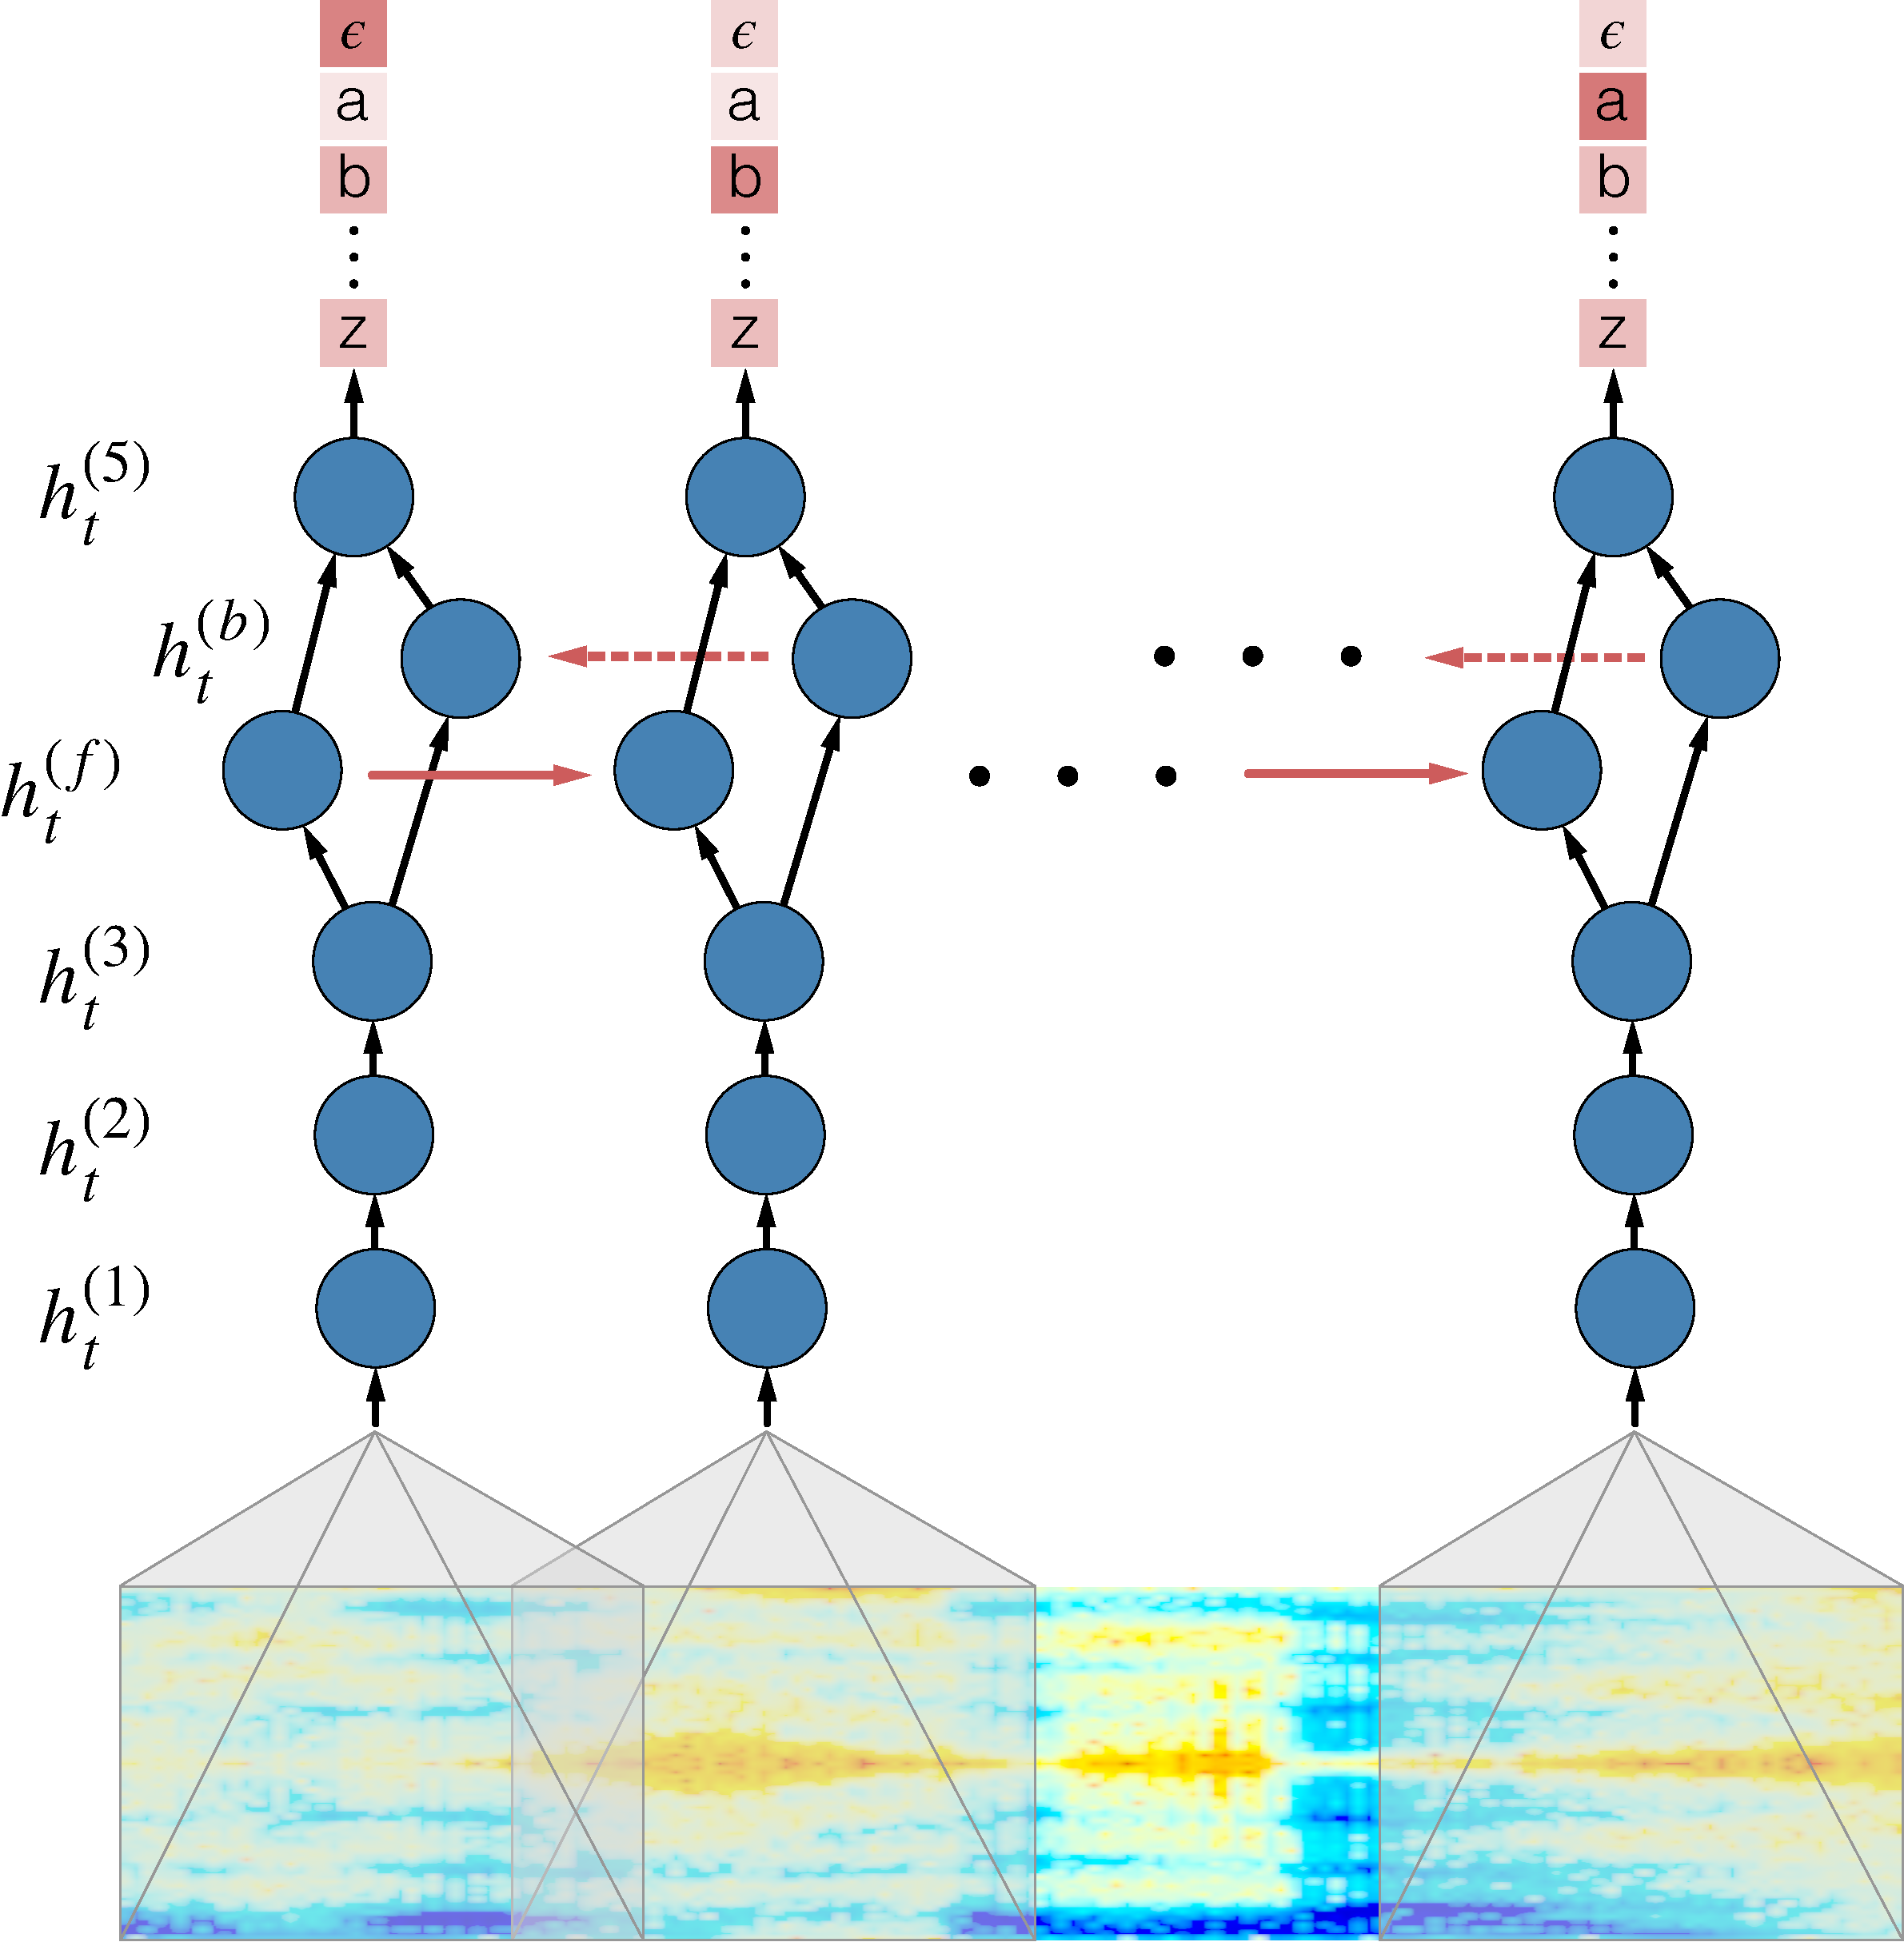
\includegraphics[width=0.6\textwidth]{deepspeech/figures/speech_network.pdf}
  \caption{Structure of our RNN model and notation.}
  \label{fig:deepspeech:rnn}
\end{figure}

The complete RNN model is illustrated in Figure~\ref{fig:deepspeech:rnn}. Note
that its structure is considerably simpler than related models from the
literature~\cite{graves2014}---we have limited ourselves to a single recurrent
layer (which is the hardest to parallelize) and we do not use
Long-Short-Term-Memory (LSTM) circuits. One disadvantage of LSTM cells is that
they require computing and storing multiple gating neuron responses at each
step. Since the forward and backward recurrences are sequential, this small
additional cost can become a computational bottleneck. By using a homogeneous
model we have made the computation of the recurrent activations as efficient as
possible: computing the ReLu outputs involves only a few highly optimized BLAS
operations on the GPU and a single point-wise nonlinearity.

\subsection{Regularization}

While we have gone to significant lengths to expand our datasets (c.f.
Section~\ref{sec:deepspeech:data}), the recurrent networks we use are still
adept at fitting the training data. In order to reduce variance further, we use
several techniques.  

During training we apply a dropout~\cite{hinton2012dropout} rate between 5\% -
10\%. We apply dropout in the feed-forward layers but not to the recurrent
hidden activations.

A commonly employed technique in computer vision during network evaluation is
to randomly jitter inputs by translations or reflections, feed each jittered
version through the network, and vote or average the
results~\cite{krizhevsky2012imagenet}. Such jittering is not common in ASR,
however we found it beneficial to translate the raw audio files by 5ms (half
the filter bank step size) to the left and right, then forward propagate the
recomputed features and average the output probabilities. At test time we also
use an ensemble of several RNNs, averaging their outputs in the same way.

\subsection{Language Model}
\label{sec:deepspeech:languagemodel}

When trained from large quantities of labeled speech data, the RNN model can
learn to produce readable character-level transcriptions. Indeed for many of
the transcriptions, the most likely character sequence predicted by the RNN is
exactly correct without external language constraints. The errors made by the
RNN in this case tend to be phonetically plausible renderings of English
words---Table~\ref{table:deepspeech:max_decoded} shows some examples. Many of
the errors occur on words that rarely or never appear in our training set. In
practice, this is hard to avoid:  training from enough speech data to
\emph{hear} all of the words or language constructions we might need to know is
impractical.  Therefore, we integrate our system with an N-gram language model
since these models are easily trained from huge unlabeled text corpora. For
comparison, while our speech datasets typically include up to 3 million
utterances, the N-gram language model used for the experiments in
Section~\ref{sec:deepspeech:expnoise} is trained from a corpus of 220 million
phrases, supporting a vocabulary of 495,000 words.\footnote{We use the KenLM
toolkit~\cite{heafield2013} to train the N-gram language models in our
experiments.} 

\begin{table}[h]
\centering
\begin{tabular}{l | l}
\toprule
RNN output  & Decoded Transcription \\
\midrule
\rule{0pt}{2ex}
what is the weather like in & what is the weather like in \\
\rule{0pt}{0.1ex}
bostin right now       & boston right now \\
\rule{0pt}{4ex}
prime miniter nerenr modi   & prime minister narendra modi \\ 
\rule{0pt}{4ex}
arther n tickets for the game  & are there any tickets for the game \\ 
\bottomrule
\end{tabular}
\caption{Examples of transcriptions directly from the RNN (left) with errors
         that are fixed by addition of a language model (right).}
\label{table:deepspeech:max_decoded}
\end{table}

We perform a search to find the sequence of characters that is most probable
according to both the RNN output and the language model (where the language
model interprets the string of characters as words). Specifically, we aim to
find a sequence $Y$ that maximizes the combined objective:
\begin{align*}
    Q(Y) = \log(p(Y \mid X)) + \alpha \log(p_{\text{lm}}(Y)) + \beta \textrm{ word\_count}(Y)
\end{align*}
where $\alpha$ and $\beta$ are tunable parameters (set by cross-validation)
that control the trade-off between the RNN, the language model constraint and
the length of the sentence. The term $p_{\text{lm}}$ denotes the
probability of the sequence $c$ according to the N-gram model. We maximize
this objective using a highly optimized beam search algorithm, with a typical
beam size in the range 1000-8000---similar to the approach described by Hannun
et al.~\cite{hannun2014firstpass}.

\section{Optimizations}
\label{sec:deepspeech:optimization}

As noted above, we have made several design decisions to make our networks
amenable to high-speed execution (and thus fast training). For example, we have
opted for homogeneous rectified-linear networks that are simple to implement
and depend on just a few highly-optimized BLAS calls. When fully unrolled, our
networks include almost 5 billion connections for a typical utterance and thus
efficient computation is critical to make our experiments feasible. We use
multi-GPU training~\cite{coates2013cotshpc, krizhevsky2012imagenet} to
accelerate our experiments, but doing this effectively requires some additional
work, as we explain.

\subsection{Data parallelism}
\label{sec:deepspeech:datapar}

In order to process data efficiently, we use two levels of data parallelism.
First, each GPU processes many examples in parallel. This is done in the usual
way by concatenating many examples into a single matrix. For instance, rather
than performing a single matrix-vector multiplication $W_r h_t$ in the
recurrent layer, we prefer to do many in parallel by computing $W_r H_t$ where
$H_t = [ h^{(i)}_{t}, h^{(i+1)}_{t}, \ldots ]$ (where $h_t^{(i)}$ corresponds
to the $i$'th example $x^{(i)}$ at time $t$). The GPU is most efficient when
$H_t$ is relatively wide (e.g., 1000 examples or more) and thus we prefer to
process as many examples on one GPU as possible (up to the limit of GPU
memory).

When we wish to use larger minibatches than a single GPU can support on its own
we use data parallelism across multiple GPUs, with each GPU processing a
separate minibatch of examples and then combining its computed gradient with
its peers during each iteration. We typically use $2\times$ or $4\times$ data
parallelism across GPUs.

Data parallelism is not easily implemented, however, when utterances have
different lengths since they cannot be combined into a single matrix
multiplication. We resolve the problem by sorting our training examples by
length and combining only similarly-sized utterances into minibatches, padding
with silence when necessary so that all utterances in a batch have the same
length. This solution is inspired by the ITPACK/ELLPACK sparse matrix
format~\cite{kincaid1989}; a similar solution was used by the Sutskever et
al.~\cite{sutskever2014} to accelerate RNNs for text.

\subsection{Model parallelism}

Data parallelism yields training speedups for modest multiples of the minibatch
size (e.g., 2 to 4), but faces diminishing returns as batching more examples
into a single gradient update fails to improve the training convergence rate.
That is, processing $2\times$ as many examples on $2\times$ as many GPUs fails
to yield a $2\times$ speedup in training. It is also inefficient to fix the
total minibatch size but spread out the examples to $2\times$ as many GPUs:  as
the minibatch \emph{within} each GPU shrinks, most operations become
memory-bandwidth limited. To scale further, we parallelize by partitioning the
model (``model parallelism''~\cite{coates2013cotshpc, dean2012}).

Our model is challenging to parallelize due to the sequential nature of the
recurrent layers. Since the bidirectional layer is comprised of a forward
computation and a backward computation that are independent, we can perform the
two computations in parallel. Unfortunately, naively splitting the RNN to place
$h^{(f)}$ and $h^{(b)}$ on separate GPUs commits us to significant data
transfers when we go to compute $h^{(5)}$ (which depends on both $h^{(f)}$ and
$h^{(b)}$). Thus, we have chosen a different partitioning of work that requires
less communication for our models: we divide the model in half along the
\emph{time} dimension.

All layers except the recurrent layer can be trivially decomposed along the
time dimension, with the first half of the time-series, from $t=1$ to
$t=T^{(i)}/2$, assigned to one GPU and the second half to another GPU. When
computing the recurrent layer activations, the first GPU begins computing the
forward activations $h^{(f)}$, while the second begins computing the backward
activations $h^{(b)}$. At the mid-point ($t=T^{(i)}/2$), the two GPUs exchange
the intermediate activations, $h^{(f)}_{T/2}$ and $h^{(b)}_{T/2}$ and swap
roles. The first GPU then finishes the backward computation of $h^{(b)}$ and
the second GPU finishes the forward computation of $h^{(f)}$.

\subsection{Striding}

We have worked to minimize the running time of the recurrent layers of our RNN,
since these are the hardest to parallelize. As a final optimization, we
shorten the recurrent layers by taking ``steps'' (or strides) of size 2 in the
original input so that the unrolled RNN has half as many steps. This is
similar to a convolutional network~\cite{lecun1989} with a step-size of 2 in
the first layer. We use the cuDNN library~\cite{chetlur2014cudnn} to implement
this first layer of convolution efficiently.

\section{Training Data}
\label{sec:deepspeech:data}

Large-scale deep learning systems require an abundance of labeled data. For our
system we need many recorded utterances and corresponding English
transcriptions, but there are few public datasets of sufficient scale. To train
our largest models we have thus collected an extensive dataset consisting of
5000 hours of read speech from 9600 speakers. For comparison, we have
summarized the labeled datasets available to us in
Table~\ref{table:deepspeech:datasets}.

\begin{table}[]
\centering
\begin{tabular}{l c c c}
 \toprule
 Dataset & Type & Hours & Speakers  \\
 \midrule
 WSJ         & read           &   80 & 280 \\
 Switchboard & conversational &  300 & 4000 \\
 Fisher      & conversational & 2000 & 23000 \\
 Baidu       & read           & 5000 & 9600 \\
 \bottomrule
\end{tabular}
\caption{A summary of the datasets used to train Deep Speech. The Wall Street
         Journal, Switchboard and Fisher~\cite{cieri2004fisher} corpora are all
         published by the Linguistic Data Consortium.}
\label{table:deepspeech:datasets}
\end{table}

\subsection{Synthesis by superposition}
\label{sec:deepspeech:noisesynth}

To expand our potential training data even further we use data synthesis, which
has been successfully applied in other contexts to amplify the effective number
of training samples~\cite{sapp2008, lecun2004, coates2011}. In our work, the
goal is primarily to improve performance in noisy environments where existing
systems break down. Capturing labeled data (e.g., read speech) from noisy
environments is not practical, however, and thus we must find other ways to
generate such data.

To a first order, audio signals are generated through a process of
superposition of source signals. We can use this fact to synthesize noisy
training data. For example, if we have a speech audio track $x^{(i)}$ and a
``noise'' audio track $\xi^{(i)}$, then we can form the ``noisy speech'' track
$\hat{x}^{(i)} = x^{(i)}+\xi^{(i)}$ to simulate audio captured in a noisy
environment. If necessary, we can add reverberations, echoes or other forms of
damping to the power spectrum of $\xi^{(i)}$ or $x^{(i)}$ and then simply add
them together to make fairly realistic audio scenes.

There are, however, some risks in this approach. For example, in order to take
1000 hours of clean speech and create 1000 hours of noisy speech, we will need
unique noise tracks spanning roughly 1000 hours. We cannot settle for, say, 10
hours of repeating noise, since it may become possible for the recurrent
network to memorize the noise track and ``subtract'' it out of the synthesized
data. Thus, instead of using a single noise source $\xi^{(i)}$ with a length of
1000 hours, we use a large number of shorter clips (which are easier to collect
from public video sources) and treat them as separate sources of noise before
superimposing all of them: $\hat{x}^{(i)} = x^{(i)} + \xi_1^{(i)} +\xi_2^{(i)}
+ \ldots$.

When superimposing many signals collected from video clips, we can end up with
``noise'' sounds that are different from the kinds of noise recorded in real
environments. To ensure a good match between our synthetic data and real data,
we rejected any candidate noise clips where the average power in each frequency
band differed significantly from the average power observed in real noisy
recordings.

\subsection{Capturing Lombard Effect}
\label{sec:deepspeech:lombard}

One challenging effect encountered by speech recognition systems in noisy
environments is the ``Lombard Effect''~\cite{junqua1993lombard}: speakers
actively change the pitch or inflections of their voice to overcome noise
around them. This (involuntary) effect does not show up in recorded speech
datasets since they are collected in quiet environments. To ensure that the
effect is represented in our training data we induce the Lombard effect
intentionally during data collection by playing loud background noise through
headphones worn by a person as they record an utterance. The noise induces them
to inflect their voice, thus allowing us to capture the Lombard effect in our
training data.\footnote{We have experimented with noise played through
headphones as well as through computer speakers. Using headphones has the
advantage that we obtain ``clean'' recordings without the background noise
included and can add our own synthetic noise afterward.}


\section{Experiments}
\label{sec:deepspeech:experiments}

We performed two sets of experiments to evaluate our system. In both cases we
use the model described in Section~\ref{sec:deepspeech:model} trained from a
selection of the datasets in Table~\ref{table:deepspeech:datasets} to predict
character-level transcriptions. The predicted probability vectors and language
model are then fed into our decoder to yield a word-level transcription, which
is compared with the ground truth transcription to yield the word error rate
(WER).

\subsection{Conversational speech: Switchboard Hub5'00 (full)}

To compare our system to prior research we use an accepted but highly
challenging test set, Hub5'00 (LDC2002S23). Some researchers split this set
into ``easy'' (Switchboard) and ``hard'' (CallHome) instances, often reporting
new results on the easier portion alone. We use the full set, which is the most
challenging case and report the overall word error rate.

We evaluate our system trained on only the 300 hour Switchboard conversational
telephone speech dataset and trained on both Switchboard (SWB) and Fisher
(FSH)~\cite{cieri2004fisher}, a 2000 hour corpus collected in a similar manner
as Switchboard. Many researchers evaluate models trained only with 300 hours
from Switchboard conversational telephone speech when testing on Hub5'00. In
part this is because training on the full 2000 hour Fisher corpus is
computationally difficult. Using the techniques mentioned in
Section~\ref{sec:deepspeech:optimization} our system is able perform a full
pass over the 2300 hours of data in just a few hours.

Since the Switchboard and Fisher corpora are distributed at a sample rate of
8kHz, we compute spectrograms of 80 linearly spaced log filter banks and an
energy term.  The filter banks are computed over windows of 20ms strided by
10ms. We did not evaluate more sophisticated features such as the mel-scale log
filter banks or the mel-frequency cepstral coefficients.

Speaker adaptation is critical to the success of current ASR
systems~\cite{vesely2013, sainath2013deep}, particularly when trained on 300
hour Switchboard. For the models we test on Hub5'00, we apply a simple form of
speaker adaptation by normalizing the spectral features on a per speaker basis.
Other than this, we do not modify the input features in any way.

For decoding, we use a 4-gram language model with a 30,000 word vocabulary
trained on the Fisher and Switchboard transcriptions. Again, hyperparameters
for the decoding objective are chosen via cross-validation on a held-out
development set.

The Deep Speech SWB model is a network of 5 hidden layers each with 2048
neurons trained on only 300 hour switchboard. The Deep Speech SWB + FSH model
is an ensemble of 4 RNNs each with 5 hidden layers of 2304 neurons trained on
the full 2300 hour combined corpus. All networks are trained on inputs of +/- 9
frames of context.

We report results in Table~\ref{table:deepspeech:hub5}. The model from Vesely
et al.  (DNN-GMM sMBR)~\cite{vesely2013} uses a sequence based loss function on
top of a DNN after using a typical hybrid DNN-HMM system to realign the
training set.  The performance of this model on the combined Hub5'00 test set
is the best previously published result. When trained on the combined 2300
hours of data the Deep Speech system improves upon this baseline by 2.4
absolute WER and 13.0\% relative. The model from Maas et al. (DNN-HMM
FSH)~\cite{maas2014} achieves 19.9 WER when trained on the Fisher 2000 hour
corpus. That system was built using Kaldi~\cite{povey2011}, state-of-the-art
open source speech recognition software. We include this result to demonstrate
that Deep Speech, when trained on a comparable amount of data is competitive
with the best existing ASR systems.

\begin{table}[ht!]
\centering
\begin{tabular}{l  c  c  c }
\toprule
Model & SWB & CH & Full \\
\midrule
Vesely et al. (GMM-HMM BMMI)~\cite{vesely2013}   & 18.6 & 33.0 & 25.8 \\
Vesely et al. (DNN-HMM sMBR)~\cite{vesely2013}    & 12.6 & 24.1  & 18.4 \\
Maas et al. (DNN-HMM SWB)~\cite{maas2014}  & 14.6 & 26.3  & 20.5 \\
Maas et al. (DNN-HMM FSH)~\cite{maas2014}  & 16.0 & 23.7  & 19.9 \\
Seide et al. (CD-DNN)~\cite{seide2011}     & 16.1 & n/a & n/a \\
Kingsbury et al. (DNN-HMM sMBR HF)~\cite{kingsbury2012}  & 13.3 & n/a & n/a \\
Sainath et al. (CNN-HMM)~\cite{sainath2013deep} & 11.5 & n/a & n/a \\
Soltau et al. (MLP/CNN+I-Vector)~\cite{soltau2014} & {\bf 10.4 } & n/a & n/a \\
{\bf Deep Speech SWB} & 20.0 & 31.8 & 25.9 \\
{\bf Deep Speech SWB + FSH} & 12.6 & {\bf 19.3} & {\bf 16.0} \\
\bottomrule
\end{tabular}
\caption{Published error rates (WER) on Switchboard dataset splits. The columns
    labeled ``SWB'' and ``CH'' are respectively the easy and hard subsets of
    Hub5'00.}
\label{table:deepspeech:hub5}
\end{table}

\subsection{Noisy speech}
\label{sec:deepspeech:expnoise}

Few standards exist for testing noisy speech performance, so we constructed our
own evaluation set of 100 noisy and 100 noise-free utterances from 10 speakers.
The noise environments included a background radio or TV; washing dishes in a
sink; a crowded cafeteria; a restaurant; and inside a car driving in the rain.
The utterance text came primarily from web search queries and text messages, as
well as news clippings, phone conversations, Internet comments, public
speeches, and movie scripts. We did not have precise control over the
signal-to-noise ratio (SNR) of the noisy samples, but we aimed for an SNR
between 2 and 6 dB. 

For the following experiments, we train our RNNs on all the datasets (more than
7000 hours) listed in Table~\ref{table:deepspeech:datasets}. Since we train for
15 to 20 epochs with newly synthesized noise in each pass, our model learns
from over 100,000 hours of novel data. We use an ensemble of 6 networks each
with 5 hidden layers of 2560 neurons. No form of speaker adaptation is applied
to the training or evaluation sets. We normalize training examples on a per
utterance basis in order to make the total power of each example consistent.
The features are 160 linearly spaced log filter banks computed over windows of
20ms strided by 10ms and an energy term. Audio files are resampled to 16kHz
prior to the featurization. Finally, from each frequency bin we remove the
global mean over the training set and divide by the global standard deviation,
primarily so the inputs are well scaled during the early stages of training.

As described in Section~\ref{sec:deepspeech:languagemodel}, we use a 5-gram
language model for the decoding. We train the language model on 220 million
phrases of the Common Crawl\footnote{commoncrawl.org}, selected such that at
least 95\% of the characters of each phrase are in the alphabet. Only the most
common 495,000 words are kept, the rest remapped to an \texttt{UNKNOWN} token.

We compared the Deep Speech system to several commercial speech systems: (1)
wit.ai, (2) Google Speech API, (3) Bing Speech and (4) Apple
Dictation.\footnote{wit.ai and Google Speech each have HTTP-based APIs. To test
Apple Dictation and Bing Speech, we used a kernel extension to loop audio
output back to audio input in conjunction with the OS X Dictation service and
the Windows 8 Bing speech recognition API.}

Our test is designed to benchmark performance in noisy environments. This
situation creates challenges for evaluating the web speech APIs: these systems
will give no result at all when the SNR is too low or in some cases when the
utterance is too long. Therefore we restrict our comparison to the subset of
utterances for which all systems returned a non-empty result.\footnote{This
leads to much higher accuracies than would be reported if we attributed 100\%
error in cases where an API failed to respond.} The results of evaluating each
system on our test files appear in Table~\ref{table:deepspeech:originalaudio}.  

To evaluate the efficacy of the noise synthesis techniques described in
Section~\ref{sec:deepspeech:noisesynth}, we trained two RNNs, one on 5000 hours
of raw data and the other trained on the same 5000 hours plus noise. On the 100
clean utterances both models perform about the same, 9.2 WER and 9.0 WER for
the clean trained model and the noise trained model respectively. However, on
the 100 noisy utterances the noisy model achieves 22.6 WER over the clean
model's 28.7 WER, a 6.1 absolute and 21.3\% relative improvement.

\begin{table}[ht!]
\centering
\begin{tabular}{l  c  c  c}
\toprule
System      &  Clean (94) &  Noisy (82) & Combined (176) \\
\midrule
Apple Dictation  & 14.24   & 43.76  & 26.73 \\
Bing Speech      &  11.73     &   36.12   &  22.05   \\
Google API       &  6.64   & 30.47  & 16.72 \\
wit.ai           &  7.94   & 35.06  & 19.41 \\
{\bf Deep Speech}       &  {\bf 6.56}   & {\bf 19.06}  & {\bf 11.85} \\
\bottomrule
\end{tabular}
\caption{Results (WER) for 5 systems evaluated on the original audio. Scores
         are reported {\it only} for utterances with predictions given by all
         systems. The number in parentheses next to each dataset, e.g. Clean (94),
         is the number of utterances scored.}
\label{table:deepspeech:originalaudio}
\end{table}




\section{Conclusion}

We have presented an end-to-end deep learning-based speech system capable of
outperforming existing state-of-the-art recognition pipelines in two
challenging scenarios: clear, conversational speech and speech in noisy
environments. Our approach is enabled particularly by multi-GPU training and by
data collection and synthesis strategies to build large training sets
exhibiting the distortions our system must handle (such as background noise and
Lombard effect). Combined, these solutions enable us to build a data-driven
speech system that is at once better performing than existing methods while no
longer relying on the complex processing stages that had stymied further
progress. We believe this approach will continue to improve as we capitalize on
increased computing power and dataset sizes in the future.


\chapter{Deep Speech 2: End-to-End Speech Recognition in English and Mandarin}

\section{Introduction}
\label{sec:deepspeech2:introduction}

Decades worth of hand-engineered domain knowledge has gone into current
state-of-the-art automatic speech recognition (ASR) pipelines. A simple but
powerful alternative solution is to train such ASR models end-to-end, using
deep learning to replace most modules with a single
model~\cite{hannun2014deepspeech}. We present the second generation of our
speech system that exemplifies the major advantages of end-to-end learning. The
{Deep Speech 2} ASR pipeline approaches or exceeds the accuracy of Amazon
Mechanical Turk human workers on several benchmarks, works in multiple
languages with little modification, and is deployable in a production setting.
It thus represents a significant step towards a single ASR system that
addresses the entire range of speech recognition contexts handled by humans.
Since our system is built on end-to-end deep learning, we can employ a spectrum
of deep learning techniques: capturing large training sets, training larger
models with high performance computing, and methodically exploring the space of
neural network architectures. We show that through these techniques we are able
to reduce error rates of our previous end-to-end
system~\cite{hannun2014deepspeech} in English by up to 43\%, and can also
recognize Mandarin speech with high accuracy.

One of the challenges of speech recognition is the wide range of variability in
speech and acoustics. As a result, modern ASR pipelines are made up of numerous
components including complex feature extraction, acoustic models, language and
pronunciation models, speaker adaptation, etc. Building and tuning these
individual components makes developing a new speech recognizer very hard,
especially for a new language. Indeed, many parts do not generalize well across
environments or languages and it is often necessary to support multiple
application-specific systems in order to provide acceptable accuracy. This
state of affairs is different from human speech recognition: people have the
innate ability to learn any language during childhood, using general skills to
learn language. After learning to read and write, most humans can transcribe
speech with robustness to variation in environment, speaker accent and noise,
without additional training for the transcription task. To meet the
expectations of speech recognition users, we believe that a single engine must
learn to be similarly competent; able to handle most applications with only
minor modifications and able to learn new languages from scratch without
dramatic changes. Our end-to-end system puts this goal within reach, allowing
us to approach or exceed the performance of human workers on several tests in
two very different languages: Mandarin and English.

Since {Deep Speech 2} (DS2) is an end-to-end deep learning system, we can
achieve performance gains by focusing on three crucial components: the model
architecture, large labeled training datasets, and computational scale. This
approach has also yielded great advances in other application areas such as
computer vision and natural language. This paper details our contribution to
these three areas for speech recognition, including an extensive investigation
of model architectures and the effect of data and model size on recognition
performance. In particular, we describe numerous experiments with neural
networks trained with the Connectionist Temporal Classification (CTC) loss
function~\cite{graves2006} to predict speech transcriptions from audio. We
consider networks composed of many layers of recurrent connections,
convolutional filters, and nonlinearities, as well as the impact of a specific
instance of Batch Normalization~\cite{ioffe2015batch} (BatchNorm) applied to
RNNs. We not only find networks that produce much better predictions than those
in previous work~\cite{hannun2014deepspeech}, but also find instances of
recurrent models that can be deployed in a production setting with no
significant loss in accuracy.

Beyond the search for better model architecture, deep learning systems benefit
greatly from large quantities of training data. We detail our data capturing
pipeline that has enabled us to create larger datasets than what is typically
used to train speech recognition systems. Our English speech system is trained
on 11,940 hours of speech, while the Mandarin system is trained on 9,400 hours.
We use data synthesis to further augment the data during training.

Training on large quantities of data usually requires the use of larger models.
Indeed, our models have many more parameters than those used in our previous
system. Training a single model at these scales requires tens of
exaFLOPs\footnote{1 exaFLOP = $10^{18}$ FLoating-point OPerations.} that would
require 3-6 weeks to execute on a single GPU. This makes model exploration a
very time consuming exercise, so we have built a highly optimized training
system that uses 8 or 16 GPUs to train one model. In contrast to previous
large-scale training approaches that use parameter servers and asynchronous
updates~\cite{dean2012, chilimbi2014}, we use synchronous SGD, which is easier
to debug while testing new ideas, and also converges faster for the same degree
of data parallelism. To make the entire system efficient, we describe
optimizations for a single GPU as well as improvements to scalability for
multiple GPUs. We employ optimization techniques typically found in High
Performance Computing to improve scalability. These optimizations include a
fast implementation of the CTC loss function on the GPU, and a custom memory
allocator. We also use carefully integrated compute nodes and a custom
implementation of all-reduce to accelerate inter-GPU communication. Overall the
system sustains approximately 50 teraFLOP/second when training on 16 GPUs. This
amounts to 3 teraFLOP/second per GPU which is about 50\% of peak theoretical
performance. This scalability and efficiency cuts training times down to 3 to 5
days, allowing us to iterate more quickly on our models and datasets.

We benchmark our system on several publicly available test sets and compare the
results to our previous end-to-end system~\cite{hannun2014deepspeech}. Our goal
is to eventually reach human-level performance not only on specific benchmarks,
where it is possible to improve through dataset-specific tuning, but on a range
of benchmarks that reflects a diverse set of scenarios. To that end, we have
also measured the performance of human workers on each benchmark for
comparison. We find that our system outperforms humans in some commonly-studied
benchmarks and has significantly closed the gap in much harder cases. In
addition to public benchmarks, we show the performance of our Mandarin system
on internal datasets that reflect real-world product scenarios.

Deep learning systems can be challenging to deploy at scale. Large neural
networks are computationally expensive to evaluate for each user utterance, and
some network architectures are more easily deployed than others. Through model
exploration, we find high-accuracy, deployable network architectures, which we
detail here. We also employ a batching scheme suitable for GPU hardware called
Batch Dispatch that leads to an efficient, real-time implementation of our
Mandarin engine on production servers. Our implementation achieves a 98th
percentile compute latency of 67 milliseconds, while the server is loaded with
10 simultaneous audio streams.

\section{Related Work}
 \label{sec:deepspeech2:related}

This work is inspired by previous work in both deep learning and speech
recognition. Feed-forward neural network acoustic models were explored more
than 20 years ago~\cite{bourlard93, renals1994, ellis1999}. Recurrent neural
networks and networks with convolution were also used in speech recognition
around the same time~\cite{robinson1996, waibel1989}. More recently DNNs have
become a fixture in the ASR pipeline with almost all state of the art speech
work containing some form of deep neural network~\cite{mohamed2011, hinton2012,
dahl2011a, dahl2011, jaitly2012, seide2011}. Convolutional networks have also
been found beneficial for acoustic models~\cite{abdelhamid2012,
sainath2013deep}. Recurrent neural networks, typically LSTMs, are just
beginning to be deployed in state-of-the art recognizers~\cite{graves2013,
sak2014, sak2014b} and work well together with convolutional layers for the
feature extraction~\cite{sainath2015}. Models with both
bidirectional~\cite{graves2013} and unidirectional recurrence have been
explored as well.

End-to-end speech recognition is an active area of research, showing compelling
results when used to re-score the outputs of a DNN-HMM~\cite{graves2014} and
standalone~\cite{hannun2014deepspeech}. Two methods are currently used to map
variable length audio sequences directly to variable length transcriptions. The
RNN encoder-decoder paradigm uses an encoder RNN to map the input to a fixed
length vector and a decoder network to expand the fixed length vector into a
sequence of output predictions~\cite{cho2014, sutskever2014}. Adding an
attentional mechanism to the decoder greatly improves performance of the
system, particularly with long inputs or outputs~\cite{bahdanau2014}. In
speech, the RNN encoder-decoder with attention performs well both in predicting
phonemes~\cite{chorowski2014} or graphemes~\cite{bahdanau2016, chan2016}. 

The other commonly used technique for mapping variable length audio input to
variable length output is the CTC loss function~\cite{graves2006} coupled with
an RNN to model temporal information. The CTC-RNN model performs well in
end-to-end speech recognition with grapheme outputs~\cite{graves2014,
hannun2014firstpass, hannun2014deepspeech, maas2015}. The CTC-RNN model has
also been shown to work well in predicting phonemes~\cite{miao2015, sak2015},
though a lexicon is still needed in this case.  Furthermore it has been
necessary to pre-train the CTC-RNN network with a DNN cross-entropy network
that is fed frame-wise alignments from a GMM-HMM system~\cite{sak2015}. In
contrast, we train the CTC-RNN networks from scratch without the need of
frame-wise alignments for pre-training.

Exploiting scale in deep learning has been central to the success of the field
thus far~\cite{krizhevsky2012imagenet, le2013}. Training on a single GPU
resulted in substantial performance gains~\cite{raina2009}, which were
subsequently scaled linearly to two~\cite{krizhevsky2012imagenet} or more
GPUs~\cite{coates2013cotshpc}. We take advantage of work in increasing
individual GPU efficiency for low-level deep learning
primitives~\cite{chetlur14}. We build on the past work in using
model-parallelism~\cite{coates2013cotshpc}, data-parallelism~\cite{dean2012} or
a combination of the two~\cite{szegedy2015, hannun2014deepspeech} to create a
fast and highly scalable system for training deep RNNs in speech recognition.

Data has also been central to the success of end-to-end speech recognition,
with over 7000 hours of labeled speech used in Deep Speech 1
(DS1)~\cite{hannun2014deepspeech}. Data augmentation has been highly effective
in improving the performance of deep learning in computer
vision~\cite{lecun2004, sapp2008, coates2011}. This has also been shown to
improve speech systems~\cite{gales2009, hannun2014deepspeech}. Techniques used
for data augmentation in speech range from simple noise
addition~\cite{hannun2014deepspeech} to complex perturbations such as
simulating changes to the vocal tract length and rate of speech of the
speaker~\cite{jaitly2013, ko2015}.

Existing speech systems can also be used to bootstrap new data collection. In
one approach, the authors use one speech engine to align and filter a thousand
hours of read speech~\cite{panayotov2015}. In another approach, a heavy-weight
offline speech recognizer is used to generate transcriptions for tens of
thousands of hours of speech~\cite{kapralova2014}. This is then passed through
a filter and used to re-train the recognizer, resulting in significant
performance gains. We draw inspiration from these past approaches in
bootstrapping larger datasets and data augmentation to increase the effective
amount of labeled data for our system.

\section{Model Architecture}
\label{sec:deepspeech2:model}

A simple multi-layer model with a single recurrent layer cannot exploit
thousands of hours of labelled speech. In order to learn from datasets this
large, we increase the model capacity via depth. We explore architectures with
up to 11 layers including many bidirectional recurrent layers and convolutional
layers. These models have nearly 8 times the amount of computation per data
example as the models in Deep Speech 1 making fast optimization and computation
critical. In order to optimize these models successfully, we use Batch
Normalization for RNNs and a novel optimization curriculum we call SortaGrad.
We also exploit long \emph{strides} between RNN inputs to reduce computation
per example by a factor of 3. This is helpful for both training and evaluation,
though requires some modifications in order to work well with CTC. Finally,
though many of our research results make use of bidirectional recurrent layers,
we find that excellent models exist using only unidirectional recurrent
layers---a feature that makes such models much easier to deploy.  Taken
together these features allow us to tractably optimize deep RNNs and improve
performance by more than 40\% in both English and Mandarin error rates over the
smaller baseline models.

\subsection{Preliminaries}

Figure~\ref{fig:deepspeech2:ds2_network} shows the architecture of the DS2
system which at its core is similar to the previous DS1
system~\cite{hannun2014deepspeech}: a recurrent neural network (RNN) trained to
ingest speech spectrograms and generate text transcriptions. 

Let a single utterance $x^{(i)}$ and label $y^{(i)}$ be sampled from a training
set $\mathcal{X} = \{(x^{(1)},y^{(1)}),(x^{(2)},y^{(2)}),\ldots\}$. Each
utterance, $x^{(i)}$, is a time-series of length $T^{(i)}$ where every
time-slice is a vector of audio features, $x_t^{(i)},  t=0,\ldots,T^{(i)}-1$.
We use a spectrogram of power normalized audio clips as the features to the
system, so $x^{(i)}_{t,p}$ denotes the power of the $p$'th frequency bin in the
audio frame at time $t$. The goal of the RNN is to convert an input sequence
$x^{(i)}$ into a final transcription $y^{(i)}$. For notational convenience, we
drop the superscripts and use $x$ to denote a chosen utterance and $y$ the
corresponding label.

The outputs of the network are the graphemes of each language. At each output
time-step $t$, the RNN makes a prediction over characters, $p(\ell_t | x)$,
where $\ell_t$ is either a character in the alphabet or the blank symbol. In
English we have $\ell_t \in \{\textrm{a, b, c, }\ldots, \textrm{z},
\textit{space}, \textit{apostrophe}, \textit{blank}\}$, where we have added the
\textit{apostrophe} as well as a \textit{space} symbol to denote word
boundaries. For the Mandarin system the network outputs simplified Chinese
characters.  We describe this in more detail in
Section~\ref{sec:deepspeech2:chinesemodel}.

\begin{figure}
    \centering
    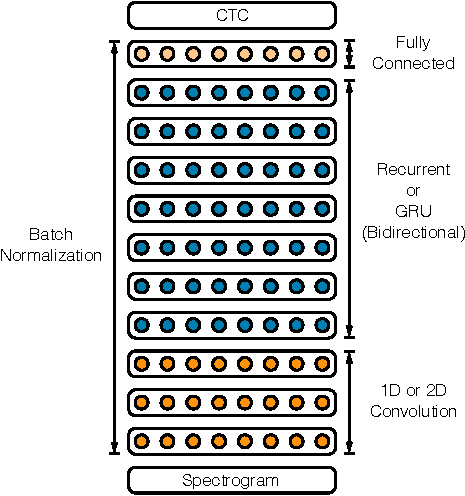
\includegraphics[width=0.6\textwidth]{deepspeech2/figures/ds2_architecture.pdf}
    \caption{The architecture of the DS2 network used for both English and
             Mandarin speech.}
    \label{fig:deepspeech2:ds2_network}
\end{figure}

The RNN model is composed of several layers of hidden units. The architectures
we experiment with consist of one or more convolutional layers, followed by one
or more recurrent layers, followed by one or more fully connected layers.

The hidden representation at layer $l$ is given by $h^l$ with the convention
that $h^0$ represents the input $x$. The bottom of the network is one or more
convolutions over the time dimension of the input. For a context window of size
$c$, the $i$-th activation at time-step $t$ of the convolutional layer is given
by
\begin{equation*}
h_{t,i}^l = f( w_i^l \circ h^{l-1}_{t-c:t+c} )
\end{equation*}
where $\circ$ denotes the element-wise product between the $i$-th filter and
the context window of the previous layers activations, and $f$ denotes a unary
nonlinear function. We use the clipped rectified-linear (ReLU) function $f(x) =
\min\{\max\{x, 0\},20\}$ as our nonlinearity. In some layers, usually the
first, we sub-sample by striding the convolution by $s$ frames. The goal is to
shorten the number of time-steps for the recurrent layers above.

Following the convolutional layers are one or more bidirectional recurrent
layers~\cite{schuster1997bidirectional}. The forward in time
$\overrightarrow{h}^l$ and backward in time $\overleftarrow{h}^l$ recurrent
layer activations are computed as
\begin{equation*}
\begin{aligned}
    \overrightarrow{h}_t^l &= g( h_t^{l-1}, \overrightarrow{h}_{t-1}^l ) \\
    \overleftarrow{h}_t^l &= g( h_t^{l-1}, \overleftarrow{h}_{t+1}^l )
\end{aligned}
\end{equation*}
The two sets of activations are summed to form the output activations for the
layer $h^l = \overrightarrow{h}^l + \overleftarrow{h}^l$.  The function
$g(\cdot)$ can be the standard recurrent operation
\begin{equation}
    \overrightarrow{h}_t^l = g( h_t^{l-1}, \overrightarrow{h}_{t-1}^l )
        = f( W^l h_t^{l-1} + \overrightarrow{U}^l \overrightarrow{h}_{t-1}^l + b^l )
    \label{eq:deepspeech2:plainrnn}
\end{equation}
where $W^l$ is the input-hidden weight matrix, $\overrightarrow{U}^l$ is the
recurrent weight matrix and $b^l$ is a bias term. In this case the input-hidden
weights are shared for both directions of the recurrence. The function
$g(\cdot)$ can also represent more complex recurrence operations such as the
Long Short-Term Memory (LSTM) units~\cite{hochreiter1997} and the gated
recurrent units (GRU)~\cite{cho2014}.

After the bidirectional recurrent layers we apply one or more fully connected layers with
\begin{equation*}
    h^l_t = f( W^l h^{l-1}_t + b^l )
\end{equation*}
The output layer $L$ is a softmax computing a probability distribution over characters given by
\begin{equation*}
    p(\ell_t=k \mid x) = \frac{\exp(w^L_k \cdot h^{L-1}_t)}{\sum_j \exp(w^L_j \cdot h^{L-1}_t)}
\end{equation*}

The model is trained using the CTC loss function~\cite{graves2006}. Given an
input-output pair $(x, y)$ and the current parameters of the network $\theta$,
we compute the loss function $\mathcal{L}(x, y; \theta)$ and its derivative
with respect to the parameters of the network $\nabla_\theta \mathcal{L}(x, y;
\theta)$. This derivative is then used to update the network parameters through
the backpropagation through time algorithm.

In the following subsections we describe the architectural and algorithmic
improvements made relative to DS1~\cite{hannun2014deepspeech}.  Unless
otherwise stated these improvements are language agnostic. We report results on
an English speaker held out development set which is an internal dataset
containing 2048 utterances of primarily read speech. All models are trained on
datasets described in Section~\ref{sec:deepspeech2:data}. We report Word Error
Rate (WER) for the English system and Character Error Rate (CER) for the
Mandarin system. In both cases we integrate a language model in a beam search
decoding step as described in Section~\ref{sec:deepspeech2:languagemodel}.


\subsection{Batch Normalization for Deep RNNs}
\label{sec:deepspeech2:bn}

To efficiently scale our model as we scale the training set, we increase the
depth of the networks by adding more hidden layers, rather than making each
layer larger. Previous work has examined doing so by increasing the number of
consecutive bidirectional recurrent layers~\cite{graves2013}. We explore Batch
Normalization (BatchNorm) as a technique to accelerate training for such
networks~\cite{ioffe2015batch} since they often suffer from optimization
issues. 

Recent research has shown that BatchNorm improves the speed of convergence of
recurrent nets, without showing any improvement in generalization
performance~\cite{laurent2016}. In contrast, we demonstrate that when applied
to very deep networks of simple RNNs on large data sets, batch normalization
substantially improves final generalization error while greatly accelerating
training. 

In a typical feed-forward layer containing an affine transformation followed by
a non-linearity $f(\cdot)$, we insert a BatchNorm transformation by applying
$f(\mathcal{B}(Wh))$ instead of $f(Wh + b)$, where
\begin{equation*}
    \mathcal{B}(x) = \gamma 
        \frac{x - \mathrm{E}[x]}{\left(\mathrm{Var}[x] + \epsilon\right)^{1/2}} + \beta.
\end{equation*}
The terms $\mathrm{E}$ and $\mathrm{Var}$ are the empirical mean and variance
over a minibatch. The bias $b$ of the layer is dropped since its effect is
cancelled by mean removal. The learnable parameters $\gamma$ and $\beta$ allow
the layer to scale and shift each hidden unit as desired. The constant
$\epsilon$ is small and positive, and is included only for numerical stability.
In our convolutional layers the mean and variance are estimated over all the
temporal output units for a given convolutional filter on a minibatch. The
BatchNorm transformation reduces \emph{internal covariate shift} by insulating
a given layer from potentially uninteresting changes in the mean and variance
of the layer's input.

We consider two methods of extending BatchNorm to bidirectional
RNNs~\cite{laurent2016}. A natural extension is to insert a BatchNorm
transformation immediately before every non-linearity.
Equation~\ref{eq:deepspeech2:plainrnn} then becomes 
\begin{equation*}
    \overrightarrow{h}^l_t =
        f( \mathcal{B}( W^l h^{l-1}_t + \overrightarrow{U}^l \overrightarrow{h}^l_{t-1} )).  
\end{equation*}
In this case the mean and variance statistics are accumulated over a single
time-step of the minibatch. The sequential dependence between time-steps
prevents averaging over all time-steps. We find that this technique does not
lead to improvements in optimization. We also tried accumulating an average
over successive time-steps, so later time-steps are normalized over all present
and previous time-steps. This also proved ineffective and greatly complicated
backpropagation.

We find that \emph{sequence-wise} normalization~\cite{laurent2016} overcomes
these issues. The recurrent computation is given by
\begin{equation*}
    \overrightarrow{h}^l_t = f( \mathcal{B}( W^l h^{l-1}_t) + \overrightarrow{U}^l \overrightarrow{h}^l_{t-1}).  
\end{equation*}

\begin{table}
\centering
\begin{tabular}{l  c  r r r  r  r r r  r}
\toprule
Architecture & Hidden Units & \multicolumn{4}{c}{Train} & \multicolumn{4}{c}{Dev}  \\
\midrule
     &  & \multicolumn{3}{c}{Baseline} & BatchNorm & \multicolumn{3}{c}{Baseline} & BatchNorm \\
\midrule
1 RNN, 5 total   & 2400 & & 10.55 & & 11.99 & & 13.55 & & 14.40 \\
3 RNN, 5 total   & 1880 & & 9.55  & & 8.29  & & 11.61 & & 10.56 \\
5 RNN, 7 total   & 1510 & & 8.59  & & 7.61  & & 10.77 & & 9.78 \\
7 RNN, 9 total   & 1280 & & 8.76  & & 7.68  & & 10.83 & & 9.52 \\
\bottomrule
\end{tabular}
\caption{Comparison of WER on a training and development set for various depths
         of RNN, with and without BatchNorm. The number of parameters is kept
         constant as the depth increases, thus the number of hidden units per layer
         decreases. All networks have 38 million parameters. The architecture ``M
         RNN, N total'' implies 1 layer of 1D convolution at the input, M
         consecutive bidirectional RNN layers, and the rest as fully-connected
         layers with N total layers in the network.}
\label{table:deepspeech2:batch_norm}
\end{table}

For each hidden unit, we compute the mean and variance statistics over all
items in the minibatch over the length of the sequence.
Figure~\ref{fig:deepspeech2:bn} shows that deep networks converge faster with
sequence-wise normalization.  Table~\ref{table:deepspeech2:batch_norm} shows
that the performance improvement from sequence-wise normalization increases
with the depth of the network, with a 12\% performance difference for the
deepest network. When comparing depth, in order to control for model size we
hold constant the total number of parameters and still see strong performance
gains. We would expect to see even larger improvements from depth if we held
constant the number of activations per layer and added layers. We also find
that BatchNorm harms generalization error for the shallowest network just as it
converges slower for shallower networks. 

The BatchNorm approach works well in training, but is difficult to implement
for a deployed ASR system, since it is often necessary to evaluate a single
utterance in deployment rather than a batch. We find that normalizing each
neuron to its mean and variance over just the sequence degrades performance.
Instead, we store a running average of the mean and variance for the neuron
collected during training, and use these for evaluation in
deployment~\cite{ioffe2015batch}. Using this technique, we can evaluate a
single utterance at a time with better results than evaluating with a large
batch.

\begin{figure}
\centering
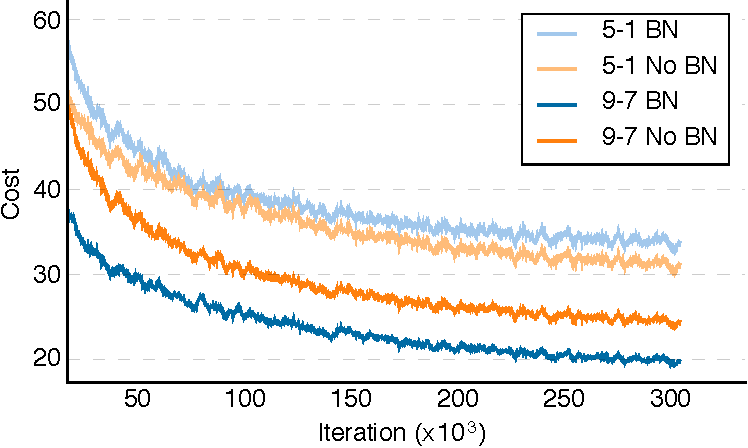
\includegraphics[width=0.6\textwidth]{deepspeech2/figures/bn_nobn.pdf}
\caption{Training curves of two models trained with and without BatchNorm. We
         start the plot after the first epoch of training as the curve is more
         difficult to interpret due to the SortaGrad curriculum.}
\label{fig:deepspeech2:bn}
\end{figure}

\subsection{SortaGrad}

Training on examples of varying length pose some algorithmic challenges. One
possible solution is truncating backpropagation through
time~\cite{williams1990}, so that all examples have the same sequence length
during training~\cite{sainath2015}. However, this can inhibit the ability to
learn longer term dependencies. Other works have found that presenting examples
in order of difficulty can accelerate online
learning~\cite{bengio2009curriculum, zaremba2014}. A common theme in many
sequence learning problems including machine translation and speech recognition
is that longer examples tend to be more challenging~\cite{cho2014}.

The CTC cost function that we use implicitly depends on the length of the
utterance,
\begin{equation}
\label{eq:deepspeech2:ctc}
    \mathcal{L}(x, y; \theta) = -\log \sum_{\ell \in \textrm{Align}(x, y)}
        \prod_t^{T} p_{\textrm{ctc}}(\ell_t \mid x; \theta).
\end{equation}
where $\textrm{Align}(x, y)$ is the set of all possible alignments of the
characters of the transcription $y$ to frames of input $x$ under the CTC
operator. In equation~\ref{eq:deepspeech2:ctc}, the inner term is a product
over time-steps of the sequence, which shrinks with the length of the sequence
since $p_{\textrm{ctc}}(\ell_t \mid x;\theta)<1$. This motivates a curriculum
learning strategy we title SortaGrad. SortaGrad uses the length of the
utterance as a heuristic for difficulty, since long utterances have higher cost
than short utterances.

\begin{table}
\centering
\begin{tabular}{l  r r r  r  r r r  r}
\toprule
& \multicolumn{4}{c}{Train} & \multicolumn{4}{c}{Dev}\\
\midrule
& \multicolumn{3}{c}{Baseline} &  BatchNorm & \multicolumn{3}{c}{Baseline} & BatchNorm\\
\midrule
Not Sorted & & 10.71 & & 8.04 & & 11.96 & & 9.78 \\
Sorted     & & 8.76 & & 7.68 & & 10.83 & & 9.52 \\
\bottomrule
\end{tabular}
\caption{Comparison of WER on a training and development set with and without
         SortaGrad, and with and without BatchNorm.}
\label{table:deepspeech2:sorting}
\end{table}

In the first training epoch, we iterate through the training set in increasing
order of the length of the longest utterance in the minibatch. After the first
epoch, training reverts back to a random order over minibatches.
Table~\ref{table:deepspeech2:sorting} shows a comparison of training cost with
and without SortaGrad on the 9 layer model with 7 recurrent layers. This effect
is particularly pronounced for networks without BatchNorm, since they are
numerically less stable. In some sense the two techniques substitute for one
another, though we still find gains when applying SortaGrad and BatchNorm
together. Even with BatchNorm we find that this curriculum improves numerical
stability and sensitivity to small changes in training. Numerical instability
can arise from different transcendental function implementations in the CPU and
the GPU, especially when computing the CTC cost. This curriculum gives
comparable results for both implementations.

We suspect that these benefits occur primarily because long utterances tend to
have larger gradients, yet we use a fixed learning rate independent of
utterance length. Furthermore, longer utterances are more likely to cause the
internal state of the RNNs to explode at an early stage in training.

\subsection{Comparison of simple RNNs and GRUs}

The models we have shown so far are \emph{simple} RNNs that have bidirectional
recurrent layers with the recurrence for both the forward in time and backward
in time directions modeled by Equation~\ref{eq:deepspeech2:plainrnn}. Current
research in speech and language processing has shown that having a more complex
recurrence can allow the network to remember state over more time-steps while
making them more computationally expensive to train~\cite{sainath2015,
chan2016, sutskever2014, bahdanau2016}. Two commonly used recurrent
architectures are the Long Short-Term Memory (LSTM)
units~\cite{hochreiter1997} and the Gated Recurrent Units
(GRU)~\cite{cho2014}, though many other variations exist. A recent
comprehensive study of thousands of variations of LSTM and GRU architectures
showed that a GRU is comparable to an LSTM with a properly initialized forget
gate bias, and their best variants are competitive with each
other~\cite{jozefowicz2015}. We decided to examine GRUs because experiments on
smaller data sets showed the GRU and LSTM reach similar accuracy for the same
number of parameters, but the GRUs were faster to train and less likely to
diverge. 

The GRUs we use are computed by 
\begin{equation*}
\begin{aligned}
z_t &= \sigma(W_z x_t + U_z h_{t-1} + b_z) \\
r_t &= \sigma(W_r x_t + U_r h_{t-1} + b_r) \\
\tilde{h}_t &= f(W_h x_t + r_t \circ U_h h_{t-1} + b_h) \\
h_t &= (1 - z_t) h_{t-1} + z_t \tilde{h}_t
\end{aligned}
\end{equation*}

where $\sigma(\cdot)$ is the sigmoid function, $z$ and $r$ represent the
\emph{update} and \emph{reset} gates respectively, and we drop the layer
superscripts for simplicity. We differ slightly from the standard GRU in that
we multiply the hidden state $h_{t-1}$ by $U_h$ prior to scaling by the reset
gate. This allows for all operations on $h_{t-1}$ to be computed in a single
matrix multiplication. The output nonlinearity $f(\cdot)$ is typically the
hyperbolic tangent function $tanh$. However, we find similar performance for
$tanh$ and clipped-ReLU nonlinearities and choose to use the clipped-ReLU for
simplicity and uniformity with the rest of the network.

\begin{table}
\centering
\begin{tabular}{l  r  r}
\toprule
Architecture &  Simple RNN & GRU \\
\midrule
5 layers, 1 Recurrent   & 14.40 & 10.53  \\
5 layers, 3 Recurrent   & 10.56 & 8.00  \\
7 layers, 5 Recurrent   & 9.78 & 7.79  \\
9 layers, 7 Recurrent   & 9.52 & 8.19  \\
\bottomrule
\end{tabular}
\caption{Comparison of development set WER for networks with either simple RNN
         or GRU, for various depths.}
\label{table:deepspeech2:rnns}
\end{table}

Both GRU and simple RNN architectures benefit from batch normalization and show
strong results with deep networks. However, Table~\ref{table:deepspeech2:rnns}
shows that for a fixed number of parameters, the GRU architectures achieve
better WER for all network depths. This is clear evidence of the long term
dependencies inherent in the speech recognition task present both within
individual words and between words. As we discuss in
Section~\ref{sec:deepspeech2:languagemodel}, even simple RNNs are able to
implicitly learn a language model due to the large amount of training data.
Interestingly, the GRU networks with 5 or more recurrent layers do not
significantly improve performance. We attribute this to the thinning from 1728
hidden units per layer for 1 recurrent layer to 768 hidden units per layer for
7 recurrent layers, to keep the total number of parameters constant.

The GRU networks outperform the simple RNNs in
Table~\ref{table:deepspeech2:rnns}. However, in later results
(Section~\ref{sec:deepspeech2:results}) we find that as we scale up the model
size, for a fixed computational budget the simple RNN networks perform slightly
better.  Given this, most of the remaining experiments use the simple RNN
layers rather than the GRUs.

\subsection{Frequency Convolutions}
\label{sec:deepspeech2:2dconv}

Temporal convolution is commonly used in speech recognition to efficiently
model temporal translation invariance for variable length utterances. This type
of convolution was first proposed for neural networks in speech more than 25
years ago~\cite{waibel1989}. Many neural network speech models have a first
layer that processes input frames with some context window~\cite{dahl2011,
vesely2013}. This can be viewed as a temporal convolution with a stride of one. 

Additionally, sub-sampling is essential to make recurrent neural networks
computationally tractable with high sample-rate audio. The DS1 system
accomplished this through the use of a spectrogram as input and temporal
convolution in the first layer with a stride parameter to reduce the number of
time-steps~\cite{hannun2014deepspeech}.

Convolutions in frequency and time domains, when applied to the spectral input
features prior to any other processing, can slightly improve ASR
performance~\cite{abdelhamid2012, sainath2013deep, soltau2014}. Convolution in
frequency attempts to model spectral variance due to speaker variability more
concisely than what is possible with large fully connected networks. Since
spectral ordering of features is removed by fully-connected and recurrent
layers, frequency convolutions work better as the first layers of the network.

We experiment with adding between one and three layers of convolution. These
are both in the time-and-frequency domain (2D invariance) and in the time-only
domain (1D invariance). In all cases we use a \emph{same} convolution,
preserving the number of input features in both frequency and time. In some
cases, we specify a stride across either dimension which reduces the size of
the output. We do not explicitly control for the number of parameters, since
convolutional layers add a small fraction of parameters to our networks. All
networks shown in Table~\ref{table:deepspeech2:2dconv} have about 35 million
parameters.

We report results on two datasets---a development set of 2048 utterances
(``Regular Dev'') and a much noisier dataset of 2048 utterances (``Noisy Dev'')
randomly sampled from the CHiME 2015 development
datasets~\cite{barker2015chime}. We find that multiple layers of 1D-invariant
convolutions provides a very small benefit. The 2D-invariant convolutions
improve results substantially on noisy data, while providing a small benefit on
clean data. The change from one layer of 1D-invariant convolution to three
layers of 2D-invariant convolution improves WER by 23.9\% on the noisy
development set.

\begin{table}
\centering
\begin{tabular}{l l l l c c c}
\toprule
Layers & Channels & Filter dimension    & Stride       & Dev         & Noisy Dev \\
\midrule
1 & 1280          & 11                  & 2             & 9.52        & 19.36 \\
2 & 640, 640      & 5, 5                & 1, 2          & 9.67        & 19.21 \\
3 & 512, 512, 512 & 5, 5, 5             & 1, 1, 2       & 9.20        & 20.22 \\
1 & 32            & 41x11               & 2x2           & 8.94        & 16.22 \\
2 & 32, 32        & 41x11, 21x11        & 2x2, 2x1      & 9.06        & 15.71 \\
3 & 32, 32, 96    & 41x11, 21x11, 21x11 & 2x2, 2x1, 2x1 & 8.61        & 14.74 \\
\bottomrule
\end{tabular}
\caption{Comparison of WER for various arrangements of convolutional layers. In
         all cases, the convolutions are followed by 7 recurrent layers and 1 fully
         connected layer. For 2D-invariant convolutions the first dimension is
         frequency and the second dimension is time.}
\label{table:deepspeech2:2dconv}
\end{table}

\subsection{Striding}

In the convolutional layers, we apply a longer stride and wider context to
speed up training as fewer time-steps are required to model a given utterance.
Downsampling the input sound (through FFT and convolutional striding) reduces
the number of time-steps and computation required in the following layers, but
at the expense of reduced performance. 

In our Mandarin models, we employ striding in the straightforward way. However,
in English, striding can reduce accuracy simply because the output of our
network requires at least one time-step per output character, and the number of
characters in English speech per time-step is high enough to cause problems
when striding\footnote{Chinese characters are more similar to English syllables
than English characters. This is reflected in our training data, where there
are on average 14.1 characters/s in English, while only 3.3 characters/s in
Mandarin. Conversely, the Shannon entropy per character as calculated from
occurrence in the training set, is less in English due to the smaller character
set---4.9 bits/char compared to 12.6 bits/char in Mandarin. This implies that
spoken Mandarin has a lower temporal entropy density, $\sim$41 bits/s compared
to $\sim$58 bits/s, and can thus more easily be temporally compressed without
losing character information.}. To overcome this, we can enrich the English
alphabet with symbols representing alternate labellings like whole words,
syllables or non-overlapping \emph{n}-grams. In practice, we use
non-overlapping bi-graphemes or bigrams, since these are simple to construct,
unlike syllables, and there are few of them compared to alternatives such as
whole words. We transform unigram labels into bigram labels through a simple
isomorphism.

Non-overlapping bigrams shorten the length of the output transcription and thus
allow for a decrease in the length of the unrolled RNN. The sentence \emph{the
cat sat} with non-overlapping bigrams is segmented as $[th, e, space, ca, t,
space, sa, t ]$. Notice that for words with odd number of characters, the last
character becomes an unigram and $space$ is treated as an unigram as well. This
isomorphism ensures that the same words are always composed of the same bigram
and unigram tokens. The output set of bigrams consists of all bigrams that
occur in the training set. 

In Table~\ref{table:deepspeech2:bigrams} we show results for both the bigram
and unigram systems for various levels of striding, with or without a language
model. We observe that bigrams allow for larger strides without any sacrifice
in in the word error rate. This allows us to reduce the number of time-steps of
the unrolled RNN benefiting both computation and memory usage.

\begin{table}
\centering
\begin{tabular}{c r r r r}
\toprule
& \multicolumn{2}{c}{Dev no LM} & \multicolumn{2}{c}{Dev LM}\\
\midrule
Stride  & Unigrams & Bigrams & Unigrams & Bigrams \\
\midrule
2 & 14.93 & 14.56 & 9.52  & 9.66  \\
3 & 15.01 & 15.60 & 9.65  & 10.06 \\
4 & 18.86 & 14.84 & 11.92 & 9.93  \\
\bottomrule
\end{tabular}
\caption{Comparison of WER with different amounts of striding for unigram and
         bigram outputs. The models are compared on a development set with and
         without the use of a 5-gram language model.}
\label{table:deepspeech2:bigrams}
\end{table}

\subsection{Row Convolution and Unidirectional Models}
\label{sec:deepspeech2:fom}

Bidirectional RNN models are challenging to deploy in an online, low-latency
setting, because they are built to operate on an entire sample, and so it is
not possible to perform the transcription process as the utterance streams from
the user. We have found an unidirectional architecture that performs as well as
our bidirectional models. This allows us to use unidirectional, forward-only
RNN layers in our deployment system. 

\begin{figure}
\centering
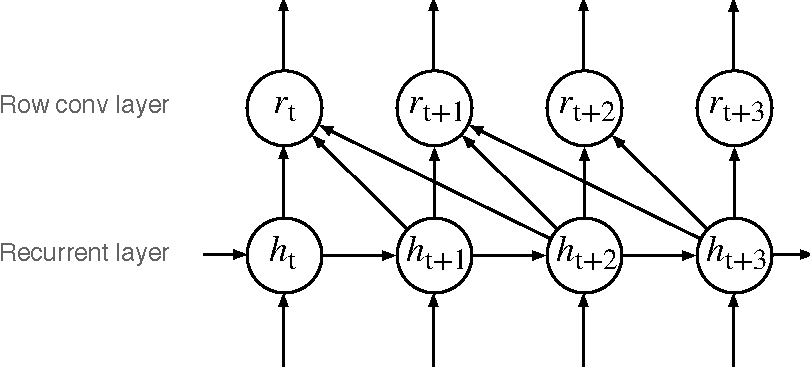
\includegraphics[width=0.6\textwidth]{deepspeech2/figures/row_conv}
\caption{The row convolution architecture with two time-steps of future context.}
\label{fig:deepspeech2:row_conv}
\end{figure}

To accomplish this, we employ a special layer that we call row convolution,
shown in Figure~\ref{fig:deepspeech2:row_conv}. The intuition behind this layer
is that we only need a small portion of future information to make an accurate
prediction at the current time-step. Suppose at time-step $t$, we use a future
context of $\tau$ steps. We now have a feature matrix $h_{t:t+\tau} = [h_t,
h_{t+1}, ..., h_{t+\tau}]$ of size $d\times(\tau+1)$. We define a parameter
matrix $W$ of the same size as $h_{t:t+\tau}$. The activations $r_t$ for the
new layer at time-step $t$ are 

\begin{align}
\label{eq:deepspeech2:rowconv}
r_{t,i} = \sum_{j=1}^{\tau+1} W_{i,j} h_{t+j-1, i}, {\rm \ for\ } 1 \leq i \leq d.
\end{align}

Since the convolution-like operation in Eq.~\ref{eq:deepspeech2:rowconv} is row
oriented for both $W$ and $h_{t:t+\tau}$, we call this layer row convolution.

We place the row convolution layer above all recurrent layers. This has two
advantages. First, this allows us to stream all computation below the row
convolution layer on a finer granularity given little future context is needed.
Second, this results in better CER compared to the best bidirectional model for
Mandarin. We conjecture that the recurrent layers have learned good feature
representations, so the row convolution layer simply gathers the appropriate
information to feed to the classifier. 

Results for a unidirectional Mandarin speech system with row convolution and a
comparison to a bidirectional model are given in
Section~\ref{sec:deepspeech2:deployment} on deployment. 

\subsection{Language Model}
\label{sec:deepspeech2:languagemodel}

We train our RNN Models over millions of unique utterances, which enables the
network to learn a powerful implicit language model. Our best models are quite
adept at spelling, without any external language constraints. Further, in our
development datasets we find many cases where our models can implicitly
disambiguate homophones---for example, ``he expects the Japanese agent
\emph{to} sell it for \emph{two} hundred seventy five thousand dollars''.
Nevertheless, the labeled training data is small compared to the size of
unlabeled text corpora that are available. Thus we find that WER improves when
we supplement our system with a language model trained from external text. 

We use an \emph{n}-gram language model since they scale well to large amounts
of unlabeled text~\cite{hannun2014deepspeech}. For English, our language model
is a Kneser-Ney smoothed 5-gram model with pruning that is trained using the
KenLM toolkit~\cite{heafield2013} on cleaned text from the Common Crawl
Repository\footnote{\url{http://commoncrawl.org}}. The vocabulary is the most
frequently used 400,000 words from 250 million lines of text, which produces a
language model with about 850 million \emph{n}-grams. For Mandarin, the
language model is a Kneser-Ney smoothed character level 5-gram model with
pruning that is trained on an internal text corpus of 8 billion lines of text.
This produces a language model with about 2 billion \emph{n}-grams.

During inference we search for the transcription $y$ that maximizes $Q(y)$
shown in Equation~\ref{eq:deepspeech2:decoding}. This is a linear combination
of $\log$ probabilities from the CTC trained network and language model, along
with a word insertion term~\cite{hannun2014deepspeech}. 

\begin{equation}
\label{eq:deepspeech2:decoding}
Q(y) = \log (p_{\textrm{ctc}}(y|x)) + \alpha \log(p_{\textrm{lm}}(y))  + \beta \: \textrm{word\_count}(y)
\end{equation}

The weight $\alpha$ controls the relative contributions of the language model
and the CTC network. The weight $\beta$ encourages more words in the
transcription. These parameters are tuned on a development set. We use a beam
search to find the optimal transcription~\cite{hannun2014firstpass}.

\begin{table}
\centering
\begin{tabular}{l  l  r r r r r r}
\toprule
Language & Architecture & \multicolumn{3}{c}{Dev no LM} & \multicolumn{3}{c}{Dev LM} \\
\midrule
English  & 5-layer, 1 RNN & & 27.79 & & & 14.39 & \\
English  & 9-layer, 7 RNN & & 14.93 & & & 9.52 & \\
Mandarin & 5-layer, 1 RNN & & 9.80  & & & 7.13 & \\
Mandarin & 9-layer, 7 RNN & & 7.55  & & & 5.81 & \\
\bottomrule
\end{tabular}
\caption{Comparison of WER for English and CER for Mandarin with and without a
         language model.}
\label{table:deepspeech2:languagemodels}
\end{table}

Table~\ref{table:deepspeech2:languagemodels} shows that an external language
model helps both English and Mandarin speech systems. The relative improvement
given by the language model drops from 48\% to 36\% in English and 27\% to 23\%
in Mandarin, as we go from a model with 5 layers and 1 recurrent layer to a
model with 9 layers and 7 recurrent layers. We hypothesize that the network
builds a stronger implicit language model with more recurrent layers. 

The relative performance improvement from a language model is higher in English
than in Mandarin. We attribute this to the fact that a Chinese character
represents a larger block of information than an English character. For
example, if we output directly to syllables or words in English, the model
would make fewer spelling mistakes and the language model would likely help
less.

\subsection{Adaptation to Mandarin}
\label{sec:deepspeech2:chinesemodel}

The techniques that we have described so far can be used to build an end-to-end
Mandarin speech recognition system that outputs Chinese characters directly.
This precludes the need to construct a pronunciation model, which is often a
fairly involved component for porting speech systems to other
languages~\cite{shan2010}. Direct output to characters also precludes the need
to explicitly model language specific pronunciation features. For example we do
not need to model Mandarin tones explicitly, as some speech systems must
do~\cite{shan2010, niu2013}.

The only architectural changes we make to our networks are due to the
characteristics of the Chinese character set. Firstly, the output layer of the
network outputs about 6000 characters, which includes the Roman alphabet, since
hybrid Chinese-English transcripts are common. We incur an out of vocabulary
error at evaluation time if a character is not contained in this set. This is
not a major concern, as our test set has only 0.74\% out of vocab characters.

We use a character level language model in Mandarin as words are not usually
segmented in text. The word insertion term of
Equation~\ref{eq:deepspeech2:decoding} becomes a character insertion term. In
addition, we find that the performance of the beam search during decoding
levels off at a smaller beam size. This allows us to use a beam size of 200
with a negligible degradation in CER. In
Section~\ref{sec:deepspeech2:results_mandarin}, we show that our Mandarin
speech models show roughly the same improvements to architectural changes as
our English speech models.

\section{Data}
\label{sec:deepspeech2:data}

Large-scale deep learning systems require an abundance of labeled training
data. We have collected an extensive training dataset for both English and
Mandarin speech models, in addition to augmenting our training with publicly
available datasets. In English we use 11,940 hours of labeled speech data
containing 8 million utterances summarized in
Table~\ref{table:deepspeech2:englishdata}.  For the Mandarin system we use
9,400 hours of labeled audio containing 11 million utterances. The Mandarin
speech data consists of internal Baidu corpora, representing a mix of read
speech and spontaneous speech, in both standard Mandarin and accented Mandarin.

\begin{table}
\centering
\begin{tabular}{l l r}
 \toprule
 Dataset & Speech Type & Hours \\
 \midrule
 WSJ          & read           &   80  \\
 Switchboard  & conversational &  300  \\
 Fisher       & conversational & 2000  \\
 LibriSpeech  & read           &  960  \\
 Baidu        & read           & 5000  \\
 Baidu        & mixed          & 3600  \\
 \midrule
 Total       &                &  11940 \\
 \bottomrule
\end{tabular}
\caption{Summary of the datasets used to train DS2 in English. The Wall Street
        Journal (WSJ), Switchboard and Fisher~\cite{cieri2004fisher} corpora are
        all published by the Linguistic Data Consortium. The LibriSpeech
        dataset~\cite{panayotov2015} is available free on-line. The other datasets
        are internal Baidu corpora.}
\label{table:deepspeech2:englishdata}
\end{table}


\subsection{Dataset Construction}

Some of the internal English (3,600 hours) and Mandarin (1,400 hours) datasets
were created from raw data captured as long audio clips with noisy
transcriptions. The length of these clips ranged from several minutes to more
than hour, making it impractical to unroll them in time in the RNN during
training. To solve this problem, we developed an alignment, segmentation and
filtering pipeline that can generate a training set with shorter utterances and
few erroneous transcriptions.

The first step in the pipeline is to use an existing bidirectional RNN model
trained with CTC to align the transcription to the frames of audio. For a given
audio-transcript pair, $(x, y)$, we find the alignment that maximizes
\begin{equation*}
\ell^* = \argmax_{\ell \in \text{Align}(x,y)} \prod_t^T p_{\text{ctc}}(\ell_t | x; \theta).
\end{equation*}
This is essentially a Viterbi alignment found using a RNN model trained with
CTC. Since Equation~\ref{eq:deepspeech2:ctc} integrates over the alignment, the
CTC loss function is never explicitly asked to produce an accurate alignment.
In principle, CTC could choose to emit all the characters of the transcription
after some fixed delay and this can happen with unidirectional
RNNs~\cite{sak2015}. However, we found that CTC produces an accurate alignment
when trained with a bidirectional RNN.

Following the alignment is a segmentation step that splices the audio and the
corresponding aligned transcription whenever it encounters a long series of
consecutive \emph{blank} labels occurs, since this usually denotes a stretch of
silence. By tuning the number of consecutive \emph{blank}s, we can tune the
length of the utterances generated. For the English speech data, we also
require a \emph{space} token to be within the stretch of \emph{blank}s in order
to segment only on word boundaries. We tune the segmentation to generate
utterances that are on average 7 seconds long.

The final step in the pipeline removes erroneous examples that arise from a
failed alignment. We crowd source the ground truth transcriptions for several
thousand examples. The word level edit distance between the ground truth and
the aligned transcription is used to produce a \emph{good} or \emph{bad} label.
The threshold for the word level edit distance is chosen such that the
resulting WER of the \emph{good} portion of the development set is less than
5\%. We then train a linear classifier to accurately predict bad examples given
the input features generated from the speech recognizer. We find the following
features useful: the raw CTC cost, the CTC cost normalized by the sequence
length, the CTC cost normalized by the transcript length, the ratio of the
sequence length to the transcript length, the number of words in the
transcription and the number of characters in the transcription. For the
English dataset, we find that the filtering pipeline reduces the WER from 17\%
to 5\% while retaining more than 50\% of the examples.

\subsection{Data Augmentation}

We augment our training data by adding noise to increase the effective size of
our training data and to improve our robustness to noisy
speech~\cite{hannun2014deepspeech}. Although the training data contains some
intrinsic noise, we can increase the quantity and variety of noise through
augmentation. Too much noise augmentation tends to make optimization difficult
and can lead to worse results, and too little noise augmentation makes the
system less robust to low signal-to-noise speech.  We find that a good balance
is to add noise to 40\% of the utterances that are chosen at random. The noise
source consists of several thousand hours of randomly selected audio clips
combined to produce hundreds of hours of noise.

\subsection{Scaling Data}

Our English and Mandarin corpora are substantially larger than those commonly
reported in speech recognition literature. In
Table~\ref{table:deepspeech2:datascale}, we show the effect of increasing the
amount of labeled training data on WER. This is done by randomly sampling the
full dataset before training. For each dataset, the model was trained for up to
20 epochs though usually early-stopped based on the error on a held out
development set. We note that the WER decreases with a power law for both the
regular and noisy development sets. The WER decreases by $\sim$40\% relative
for each factor of 10 increase in training set size. We also observe a
consistent gap in WER ($\sim$60\% relative) between the regular and noisy
datasets, implying that more data benefits both cases equally. 

This implies that a speech system will continue to improve with more labeled
training data. We hypothesize that equally as important as increasing raw
number of hours is increasing the number of speech \emph{contexts} that are
captured in the dataset. A context can be any property that makes speech unique
including different speakers, background noise, environment, and microphone
hardware. While we do not have the labels needed to validate this claim, we
suspect that measuring WER as a function of speakers in the dataset would lead
to much larger relative gains than simple random sampling.

\begin{table}
\centering
\begin{tabular}{r r r  r  r r r  r r r}
\toprule
\multicolumn{3}{c}{Fraction of Data} & Hours & \multicolumn{3}{c}{Regular Dev} & \multicolumn{3}{c}{Noisy Dev} \\
\midrule
& 1\%   & & 120   & & 29.23 & & & 50.97 & \\
& 10\%  & & 1200  & & 13.80 & & & 22.99 & \\
& 20\%  & & 2400  & & 11.65 & & & 20.41 & \\
& 50\%  & & 6000  & & 9.51  & & & 15.90 & \\
& 100\% & & 12000 & & 8.46  & & & 13.59 & \\
\bottomrule
\end{tabular}
\caption{Comparison of English WER for Regular and Noisy development sets on
         increasing training dataset size. The architecture is a 9-layer model with
         2 layers of 2D-invariant convolution and 7 recurrent layers with 68M
         parameters.}
\label{table:deepspeech2:datascale}
\end{table}

\section{Results}
\label{sec:deepspeech2:results}

To better assess the real-world applicability of our speech system, we evaluate
on a wide range of test sets. We use several publicly available benchmarks and
several test sets collected internally. Together these test sets represent a
wide range of challenging speech environments including low signal-to-noise
ratios (noisy and far-field), accented, read, spontaneous and conversational
speech. 

All models are trained for 20 epochs on either the full English dataset,
described in Table~\ref{table:deepspeech2:englishdata}, or the full Mandarin
dataset described in Section~\ref{sec:deepspeech2:data}. We use stochastic
gradient descent with Nesterov momentum~\cite{sutskever2013} along with a
minibatch of 512 utterances. If the norm of the gradient exceeds a threshold of
400, it is rescaled to 400~\cite{pascanu2013}. The model which performs the
best on a held-out development set during training is chosen for evaluation.
The learning rate is chosen from $[1\times10^{-4}, 6\times10^{-4}]$ to yield
fastest convergence and annealed by a constant factor of 1.2 after each epoch.
We use a momentum of 0.99 for all models.

The language models used are those described in
Section~\ref{sec:deepspeech2:languagemodel}. The decoding parameters from
Equation~\ref{eq:deepspeech2:decoding} are tuned on a held-out development set.
We use a beam size of 500 for the English decoder and a beam size of 200 for
the Mandarin decoder.

\subsection{English}
\label{sec:deepspeech2:english_results}

The best DS2 model has 11 layers with 3 layers of 2D convolution, 7
bidirectional recurrent layers, a fully-connected output layer along with Batch
Normalization. The first layer outputs to bigrams with a temporal stride of 3.
By comparison the DS1 model has 5 layers with a single bidirectional recurrent
layer and it outputs to unigrams with a temporal stride of 2 in the first
layer. We report results on several test sets for both the DS2 and DS1 model.
We do not tune or adapt either model to any of the speech conditions in the
test sets. Language model decoding parameters are set once on a held-out
development set.

To put the performance of our system in context, we benchmark most of our
results against human workers, since speech recognition is an audio perception
and language understanding problem that humans excel at. We obtain a measure of
human level performance by paying workers from Amazon Mechanical Turk to
hand-transcribe all of our test sets. Two workers transcribe the same audio
clip, that is typically about 5 seconds long, and we use the better of the two
transcriptions for the final WER calculation. They are free to listen to the
audio clip as many times as they like. These workers are mostly based in the
United States, and on average spend about 27 seconds per transcription. The
hand-transcribed results are compared to the existing ground truth to produce a
WER. While the existing ground truth transcriptions do have some label error,
this is rarely more than 1\%. This implies that disagreement between the ground
truth transcripts and the human level transcripts is a good heuristic for human
level performance.

\subsubsection{Model Size}

Our English speech training set is substantially larger than the size of
commonly used speech datasets. Furthermore, the data is augmented with noise
synthesis. To get the best generalization error, we expect that the model size
must increase to fully exploit the patterns in the data. In
Section~\ref{sec:deepspeech2:bn} we explored the effect of model depth while
fixing the number of parameters. In contrast, here we show the effect of
varying model size on the performance of the speech system. We only vary the
size of each layer, while keeping the depth and other architectural parameters
constant. We evaluate the models on the same Regular and Noisy development sets
that we use in Section~\ref{sec:deepspeech2:2dconv}.

\begin{table}
\centering
\begin{tabular}{r  c  r r r  r r r}
\toprule
Model size & Model type & \multicolumn{3}{c}{Regular Dev} & \multicolumn{3}{c}{Noisy Dev} \\
\midrule
$18  \times 10^6$    & GRU &   & 10.59 & &  & 21.38 & \\
$38  \times 10^6$    & GRU &   & 9.06  & &  & 17.07 & \\
$70  \times 10^6$    & GRU &   & 8.54  & &  & 15.98 & \\
$70  \times 10^6$    & RNN &   & 8.44  & &  & 15.09 & \\
$100 \times 10^6$    & GRU &   & 7.78  & &  & 14.17 & \\
$100 \times 10^6$    & RNN &   & 7.73  & &  & 13.06 & \\
\bottomrule
\end{tabular}
\caption{Comparing the effect of model size on the WER of the English speech
    system on both the regular and noisy development sets. We vary the number
    of hidden units in all but the convolutional layers. The GRU model has 3
    layers of bidirectional GRUs with 1 layer of 2D-invariant convolution. The
    RNN model has 7 layers of bidirectional simple recurrence with 3 layers of
    2D-invariant convolution. Both models output bigrams with a temporal stride
    of 3. All models contain approximately 35 million parameters and are
    trained with BatchNorm and SortaGrad.}
\label{table:deepspeech2:modelsize}
\end{table}

The models in Table~\ref{table:deepspeech2:modelsize} differ from those in
Table~\ref{table:deepspeech2:rnns} in that we increase the the stride to 3 and
output to bigrams. Because we increase the model size to as many as 100 million
parameters, we find that an increase in stride is necessary for fast
computation and memory constraints. However, in this regime we note that the
performance advantage of the GRU networks appears to diminish over the simple
RNN. In fact, for the 100 million parameter networks the simple RNN performs
better than the GRU network and is faster to train despite the 2 extra layers
of convolution.

Table~\ref{table:deepspeech2:modelsize} shows that the performance of the
system improves consistently up to 100 million parameters. All further English
DS2 results are reported with this same 100 million parameter RNN model since
it achieves the lowest generalization errors.

Table~\ref{table:deepspeech2:test} shows that the 100 million parameter RNN
model (DS2) gives a 43.4\% relative improvement over the 5-layer model with 1
recurrent layer (DS1) on an internal Baidu dataset of 3,300 utterances that
contains a wide variety of speech including challenging accents, low
signal-to-noise ratios from far-field or background noise, spontaneous and
conversational speech. 

\begin{table}
\centering
\begin{tabular}{l  c  c  c}
\toprule
Test set   & DS1 & DS2 \\
\midrule
Baidu Test & 24.01  & 13.59 \\
\bottomrule
\end{tabular}
\caption{Comparison of DS1 and DS2 WER on an internal test set of 3,300
    examples. The test set contains a wide variety of speech including accents,
    low signal-to-noise speech, spontaneous and conversational speech.}
\label{table:deepspeech2:test}
\end{table}

\subsubsection{Read Speech}

Read speech with high signal-to-noise ratio is arguably the easiest large
vocabulary for a continuous speech recognition task. We benchmark our system on
two test sets from the Wall Street Journal (WSJ) corpus of read news articles.
These are available in the LDC catalog as LDC94S13B and LDC93S6B. We also take
advantage of the recently developed LibriSpeech corpus constructed using audio
books from the LibriVox project~\cite{panayotov2015}.

Table~\ref{table:deepspeech2:readspeech} shows that the DS2 system outperforms
humans in 3 out of the 4 test sets and is competitive on the fourth. Given this
result, we suspect that there is little room for a generic speech system to
further improve on clean read speech without further domain adaptation.

\begin{table}
\centering
\begin{tabular}{l  r  r r}
\toprule
\multicolumn{4}{c}{Read Speech}\\
\midrule
Test set               & DS1   & DS2 &  Human \\ 
\midrule
WSJ eval'92            & 4.94  & 3.60  & 5.03 \\ 
WSJ eval'93            & 6.94  & 4.98  & 8.08 \\ 
LibriSpeech test-clean & 7.89  & 5.33  & 5.83 \\ 
LibriSpeech test-other & 21.74 & 13.25 & 12.69 \\ 
\bottomrule
\end{tabular}
\caption{Comparison of WER for two speech systems and human level performance
         on read speech.}
\label{table:deepspeech2:readspeech}
\end{table}

\subsubsection{Accented Speech}

Our source for accented speech is the publicly available
VoxForge\footnote{\url{http://www.voxforge.org}} dataset, which has clean
speech read from speakers with many different accents. We group these accents
into four categories. The American-Canadian and Indian groups are
self-explanatory. The Commonwealth accent denotes speakers with British, Irish,
South African, Australian and New Zealand accents. The European group contains
speakers with accents from countries in Europe that do not have English as a
first language.  We construct a test set from the VoxForge data with 1024
examples from each accent group for a total of 4096 examples.

Performance on these test sets is to some extent a measure of the breadth and
quality of our training data. Table~\ref{table:deepspeech2:voxforge} shows that
our performance improved on all the accents when we include more accented
training data and use an architecture that can effectively train on that data.
However human level performance is still notably better than that of DS2 for
all but the Indian accent. 

\begin{table}
\centering
\begin{tabular}{l  r  r  r}
\toprule
\multicolumn{4}{c}{Accented Speech}\\
\midrule
Test set                   & DS1   & DS2 & Human \\
\midrule
VoxForge American-Canadian & 15.01 & 7.55  & 4.85 \\
VoxForge Commonwealth      & 28.46 & 13.56 & 8.15 \\
VoxForge European          & 31.20 & 17.55 & 12.76 \\
VoxForge Indian            & 45.35 & 22.44 & 22.15 \\
\bottomrule
\end{tabular}
\caption{Comparing WER of the DS1 system to the DS2 system on accented speech.}
\label{table:deepspeech2:voxforge}
\end{table}

\subsubsection{Noisy Speech}

We test our performance on noisy speech using the publicly available test sets
from the recently completed third CHiME challenge~\cite{barker2015chime}. This
dataset has 1320 utterances from the WSJ test set read in various noisy
environments, including a bus, a cafe, a street and a pedestrian area. The
CHiME set also includes 1320 utterances with simulated noise from the same
environments as well as the control set containing the same utterances
delivered by the same speakers in a noise-free environment. Differences between
results on the control set and the noisy sets provide a measure of the
network's ability to handle a variety of real and synthetic noise conditions.
The CHiME audio has 6 channels and using all of them can provide substantial
performance improvements~\cite{yoshioka2015}. We use a {\it single} channel for
all our results, since multi-channel audio is not pervasive on most devices.
Table~\ref{table:deepspeech2:chime} shows that DS2 substantially improves upon
DS1, however DS2 is worse than human level performance on noisy data. The
relative gap between DS2 and human level performance is larger when the data
comes from a real noisy environment instead of synthetically adding noise to
clean speech.

\begin{table}
\centering
\begin{tabular}{l  r  r r}
\toprule
\multicolumn{4}{c}{Noisy Speech}\\
\midrule
Test set & DS1 & DS2  &  Human \\
\midrule
CHiME eval clean & 6.30  & 3.34  & 3.46 \\
CHiME eval real  & 67.94 & 21.79 & 11.84 \\
CHiME eval sim   & 80.27 & 45.05 & 31.33 \\
\bottomrule
\end{tabular}
\caption{Comparison of DS1 and DS2 system on noisy speech. ``CHiME eval clean''
         is a noise-free baseline. The ``CHiME eval real'' dataset is collected in
         real noisy environments and the ``CHiME eval sim'' dataset has similar
         noise synthetically added to clean speech.}
\label{table:deepspeech2:chime}
\end{table}

\subsection{Mandarin}
\label{sec:deepspeech2:results_mandarin}

In Table~\ref{table:deepspeech2:results_mandarin} we compare several
architectures trained on the Mandarin Chinese speech, on a development set of
2000 utterances as well as a test set of 1882 examples of noisy speech. This
development set was also used to tune the decoding parameters We see that the
deepest model with 2D-invariant convolution and BatchNorm outperforms the
shallow RNN by 48\% relative, thus continuing the trend that we saw with the
English system---multiple layers of bidirectional recurrence improves
performance substantially. 

\begin{table}[ht!]
\centering
\begin{tabular}{l  r  r  }
\toprule
Architecture & Dev & Test \\
\midrule
5-layer, 1 RNN                & 7.13  & 15.41 \\
5-layer, 3 RNN                & 6.49  & 11.85 \\
5-layer, 3 RNN + BatchNorm           & 6.22  & 9.39 \\
9-layer, 7 RNN + BatchNorm + 2D conv & 5.81  & 7.93 \\
\bottomrule
\end{tabular}
\caption{The effect of the DS2 architecture on Mandarin WER. The development
         and test sets are Baidu internal corpora.}
\label{table:deepspeech2:results_mandarin}
\end{table}

We find that our best Mandarin Chinese speech system transcribes short
voice-query like utterances better than a typical Mandarin Chinese speaker. To
benchmark against humans we ran a test with 100 randomly selected utterances
and had a group of 5 humans label all of them together. The group of humans had
an error rate of 4.0\% as compared to the speech systems performance of 3.7\%.
We also compared a single human transcriber to the speech system on 250
randomly selected utterances. In this case the speech system performs much
better: 9.7\% for the human compared to 5.7\% for the speech model.

\section{Conclusion}

End-to-end deep learning presents the exciting opportunity to improve speech
recognition systems continually with increases in data and computation.
Indeed, our results show that, compared to the previous incarnation, Deep
Speech has significantly closed the gap in transcription performance with human
workers by leveraging more data and larger models. Further, since the approach
is highly generic, we've shown that it can quickly be applied to new languages.
Creating high-performing recognizers for two very different languages, English
and Mandarin, required essentially no expert knowledge of the languages.
Finally, we have also shown that this approach can be efficiently deployed by
batching user requests together on a GPU server, paving the way to deliver
end-to-end Deep Learning technologies to users. 

To achieve these results, we have explored various network architectures,
finding several effective techniques: enhancements to numerical optimization
through SortaGrad and Batch Normalization, evaluation of RNNs with larger
strides with bigram outputs for English, searching through both bidirectional
and unidirectional models. This exploration was powered by a well optimized,
High Performance Computing inspired training system that allows us to train
new, full-scale models on our large datasets in just a few days.

Overall, we believe our results confirm and exemplify the value of end-to-end
Deep Learning methods for speech recognition in several settings. In those
cases where our system is not already comparable to humans, the difference has
fallen rapidly, largely because of application-agnostic Deep Learning
techniques. We believe these techniques will continue to scale, and thus
conclude that the vision of a single speech system that outperforms humans in
most scenarios is imminently achievable.



\chapter{Conclusions}

This is the conclusion.


%\appendix
%\include{appendix1}

\bibliographystyle{plain}
\bibliography{refs}

\end{document}

